\chapter{Mounted Cardiac Sample Imaging Experimentation}

Experimentation conducted to accommodate the mesoSPIM microscope imaging of sliced and left ventricle  section samples of leporine cardiac tissue will be detailed in this chapter. Emphasis will be placed on the mounting experimentation conducted for sliced tissues due to the greater number of technical challenges faced compared to mounting LV section samples which are a better fit to the kind of three dimensional, mesoscale sized samples the system was originally designed to handle.  

The characterization of mesoscale images captured, using different designs for both sliced and LV section samples, will showcase the significant impact mount design can have on the quality of sliced tissue images obtained in the system. It is because of this impact that much attention was made through the course of experimentation on finding the optimal dimensional configurations and additive 3D printing settings/designs to achieve the mount fabrication precision necessary to successfully image tissues with minimal aberrations or astigmatisms in the generated image stacks.

\section{Tissue Mounting Methodologies}
\subsection{Sliced Tissue Sample Mounting}

The challenge faced in the mounting of sliced cleared tissues stems from the fact that the mesoSPIM system was designed for the imaging of mesoscale, structurally rigid, three dimensional samples []. This makes use of the system to image thin, structurally plastic, sliced samples complicated to achieve. To successfully image sliced samples utilizing the mesoSPIM system, the following requirements must be met by the method in which a sample is mounted onto the system in order for successfully structural imaging to proceed: 

\begin{itemize}
    \item Prevents the occurrence of motion artifacts as the sample moves in highly viscous RIMS
    \item Eliminates warping of the sample that emerges from CLARITY tissue clearing process
    \item Keeps samples immersed in RIMS without risk of leak, contamination or evaporation.
    \item Removes air pockets, bubbles which can negatively impact the imaging of the sample
\end{itemize}

To this end, 3D printed spacer mounts were utilized to mount sliced tissues. The use of Poly-lactic Acid (PLA) 3D print fabrication allowed for cost effective, mass production of multiple mounts of identical quality in short time periods compared to the metal milling or plastic casting methods available. Fast, high throughput fabrication of mounts was also essential to allow for multiple mount design iterations to be tested concurrently alongside previously established mount designs. This iteration of the design and printer settings utilized allowed for fine adjustment of both to obtain optimal results in short time spans. The process of continued mount design iterating was conducted until the end product was found via image characterization testing to reliably and sufficiently address the aforementioned challenges faced when imaging sliced tissues. 

The mount designs used in all sliced tissue data acquired and presented here will de detailed in the following section. All mount iterations, including those tested but not used for data acquisition through the course of this project are detailed in Appendix A. This includes discussion of changes made between each major generation of mount design leading to the final design selected for use in the imaging pipeline.


\subsubsection{\textit{Finalized Custom 3D Printed Spacer Design}}

\begin{figure}[H]
    \centering
    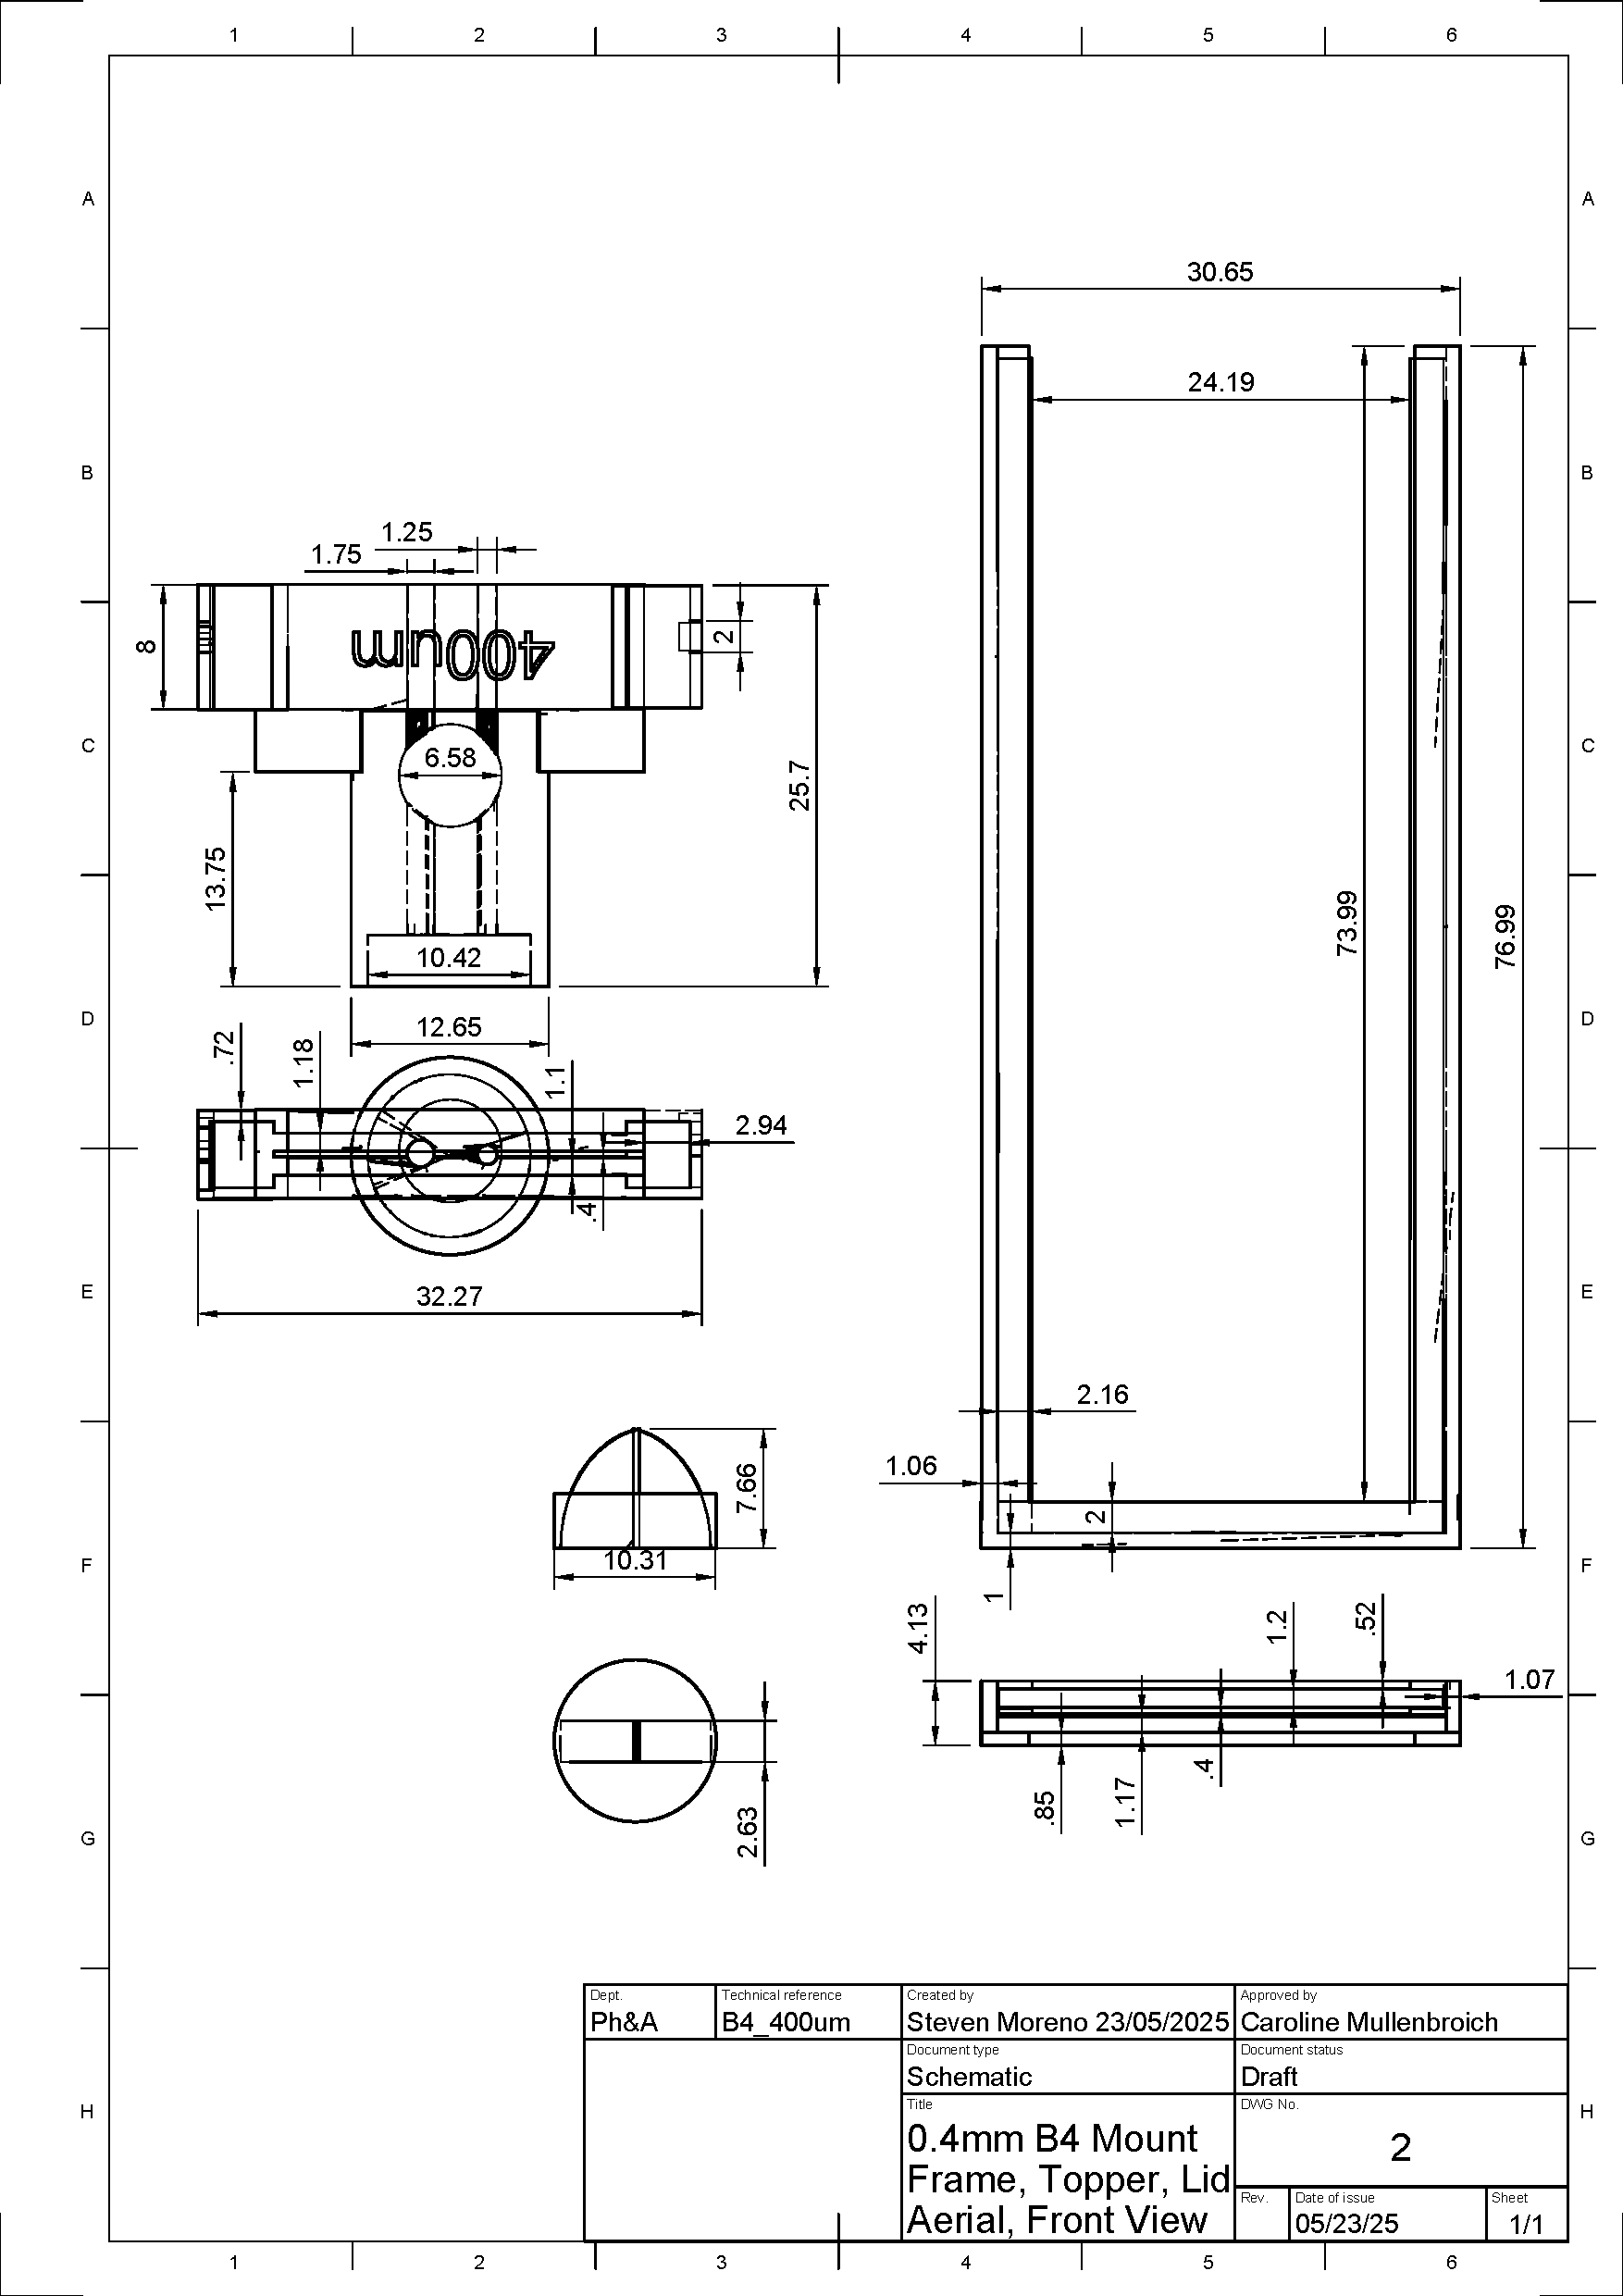
\includegraphics[width=0.5\linewidth]{Figures/0.4mm B4 Schematic v1.pdf}
    \caption{\textbf{Schematics of finalized mount design.} Mount shown is 0.4 mm internal spacer version. Designs with 0.5, 1.0, and 2.0 mm internal spacers available in Appendix A. Schematics created using Autodesk Fusion 360 software.}
    \label{fig:enter-label}
\end{figure}

The schematic and photo shown in Figure 4.1 is the finalized design of the spacer mount created for use in the imaging pipeline. Schematics for the mounts of this design with 0.5, 1.0, and 2.0 mm internal spacers are provided in Appendix A. 3D printer scripts to fabricate these mounts are available in [INSERT GITHUB URL HERE].

\subsubsection{\textit{Sliced Tissue Mounting Assembly Protocol}}

Once tissues in the imaging pipeline have completed all necessary or desired tissue staining, fixation, and washing (see Chapter 5 for protocols) the cleared tissues are placed into sealed containers wrapped in aluminium foil to protect the light sensitive fluorescent dye (if any) inside the sample.  Samples are then transported to a wet lab area adjacent to the mesoSPIM system for preparation to image. 

Lights are dimmed to the lowest possible level I could safely work in and the samples are removed from containers into a petri dish. Protective coat and gloves were put on before then proceeding with the following step by step protocol for the mounting of cleared slices into the custom designed 3D printed spacers:

\begin{figure}[H]

\begin{subfigure}{.4\linewidth}
  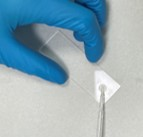
\includegraphics[width=\linewidth]{Images/Step1.jpg}
  \caption{Spread Drop of EI Solution onto slide }
  \label{MLEDdet}
\end{subfigure}\hfill 
~ 
\begin{subfigure}{.4\linewidth}
  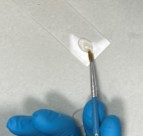
\includegraphics[width=\linewidth]{Images/Step2.jpg}
  \caption{Lay tissue slice flat atop EI drop on slide}
  \label{energydetPSK}
\end{subfigure}\hfill 

\medskip 
\begin{subfigure}{.4\linewidth}
  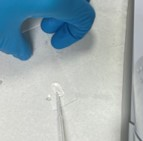
\includegraphics[width=\linewidth]{Images/Step3.jpg}
  \caption{Spread second drop of EI on top of slice}
  \label{velcomp}
\end{subfigure}\hfill 
~
\begin{subfigure}{.4\linewidth}
  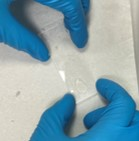
\includegraphics[width=\linewidth]{Images/Step4.jpg}
  \caption{Lay second slide atop, avoiding bubbles}
  \label{estcomp}
\end{subfigure}\hfill 

\end{figure}

\clearpage

\begin{figure}[H]
    \addtocounter{figure}{-1}

\begin{subfigure}{.4\linewidth}
\addtocounter{subfigure}{4}
  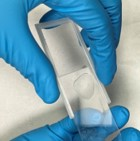
\includegraphics[width=\linewidth]{Images/Step5.jpg}
  \caption{Slide sandwiched sample into mount with internal spacer placed between the slides}
  \label{velcomp}
\end{subfigure}\hfill 
~
\begin{subfigure}{.4\linewidth}
  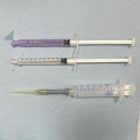
\includegraphics[width=\linewidth]{Images/Step6.jpg}
  \caption{Attach mixing nozzle, pipette tip to syringe, fill with dual-component silicone}
  \label{estcomp}
\end{subfigure}\hfill 

\medskip
\begin{subfigure}{.4\linewidth}
  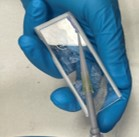
\includegraphics[width=\linewidth]{Images/Step7.jpg}
  \caption{Add mixed silicone at mount frame edges, let dry 10-15 minutes}
  \label{velcomp}
\end{subfigure}\hfill 
~
\begin{subfigure}{.4\linewidth}
  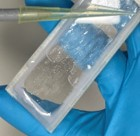
\includegraphics[width=\linewidth]{Images/Step8.jpg}
  \caption{Repeat step (g) on opposite side of mount, confirm both sides fully dried}
  \label{estcomp}
\end{subfigure}\hfill 
    
\begin{subfigure}{.4\linewidth}
  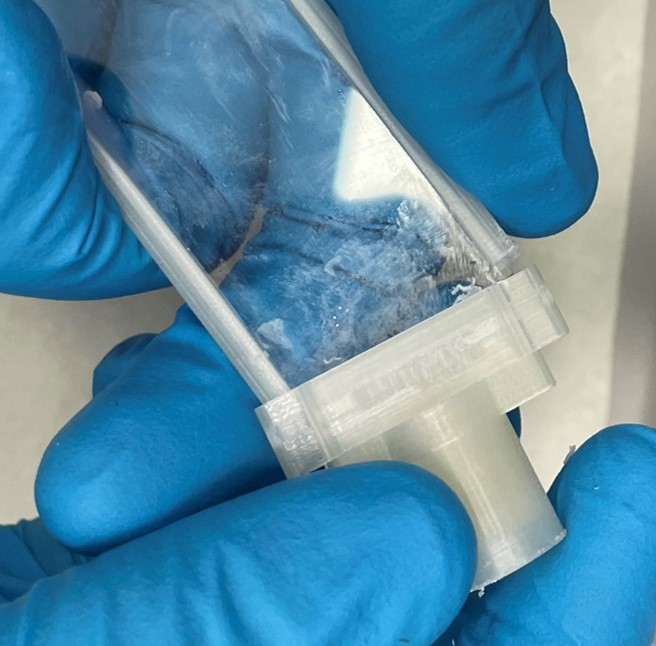
\includegraphics[width=\linewidth]{Images/Step9.jpg}
  \caption{Insert mount topper over open end of mount, ensure fully inserted}
  \label{velcomp}
\end{subfigure}\hfill 
~
\medskip
\begin{subfigure}{.4\linewidth}
  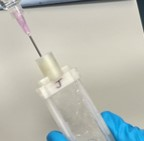
\includegraphics[width=\linewidth]{Images/Step10.jpg}
  \caption{Inject RI Matching Solution slowly via syringe port. Inject till sample immersed.}
  \label{estcomp}
\end{subfigure}\hfill 

\end{figure}

\clearpage

\begin{figure}[H]
    \addtocounter{figure}{-1}

\begin{subfigure}{.4\linewidth}
\addtocounter{subfigure}{10}
  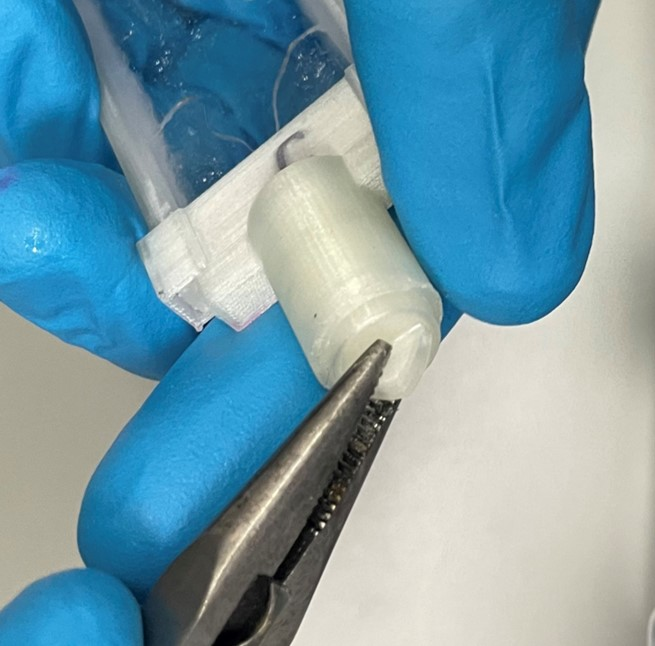
\includegraphics[width=\linewidth]{Images/Step11.jpg}
  \caption{Insert Cap over syringe ports using pliers, ensure fully inserted}
  \label{velcomp}
\end{subfigure}\hfill 
~
\medskip
\begin{subfigure}{.4\linewidth}
  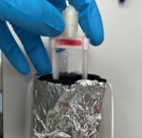
\includegraphics[width=\linewidth]{Images/Step12.jpg}
  \caption{Place mount into light protected storage for duration of RI matching period (12-24hrs).}
  \label{estcomp}
\end{subfigure}\hfill 

 \caption{\textbf{Slice Tissue Mount Assembly Procedure.} Procedure is performed with gloves to prevent smears on quartz glass, contamination of cleared samples. Mount topper marked with red and blue marks to distinguish front and back of mount for imaging.}
    \label{fig:enter-label}
\end{figure}

The protocol described in Figure 4.2 used quartz slides cleaned beforehand with ethanol solution and deionized water. Slides re-cleaned with optical cleaning tissues after mount assembly for optimal imaging. Syringe needles are disposed of in sharps bin and any EasyIndex solution residue is thoroughly cleaned using isopropanol solution. Mixing nozzles used in this protocol were 3D printed and are available on the project GITHUB repository (URL HERE). Mounts under fabrication were placed carefully in cardboard boxes with lids closed for steps requiring drying of silicone to occur to completion.



\subsection{Left Ventricle Sample Mounting}
\subsubsection{\textit{Custom 3D Printed Inner Cuvette Holder Design}}

To attach a rectangular cuvette onto the suspended sample gantry requires the development of an adapter capable of attaching the cuvette to a magnetic Thorlabs kinematic base (Thorlabs KB25/M) without risk of the cuvette detaching from the mount or cracking as a result of excessive stress applied by the mount onto the cuvette. Preliminary 3D printed, PLA mount designs consisted of a simple mount adapter that would use two nylon M2.5 screws inserted on one side of the mount to pin the cuvette wall between the flatten screw tips and the internal surface of the mount that reached partway into the cuvette internal volume. Persistent issues with this design included frequent failures of the screws to hold the sample in place and the gradual reduction in static friction over a period of time due to repeated insertion and removal of the cuvette. Damage to the walls of the cuvette were also frequent as a result of overly tight placement of nylon screws. This would lead to the formation of tension cracks on the cuvette walls.

To eliminate these issues, an additional component was added to the mount adapter: A custom designed, 3D printed base platform. This component, shown below in Figure 4.2(a), is placed beneath the cuvette, holding it in place with a rectangular notch on the platform surface. The platform attaches to the mount via four columns located at each corner of the cuvette. The columns span the height of the cuvette and connect to the upper half of the mount (Figure 4.2(b)) using M2.5 screws. The addition of this component, which avoids direct contact with the cuvette walls to suspend from above, allows for the mounting of the cuvette to occur with minimal risk of damage to the cuvette or detachment from the sample gantry. 

\begin{figure}[H]
    \centering
    \begin{subfigure}[b]{0.6\textwidth}
    \centering
    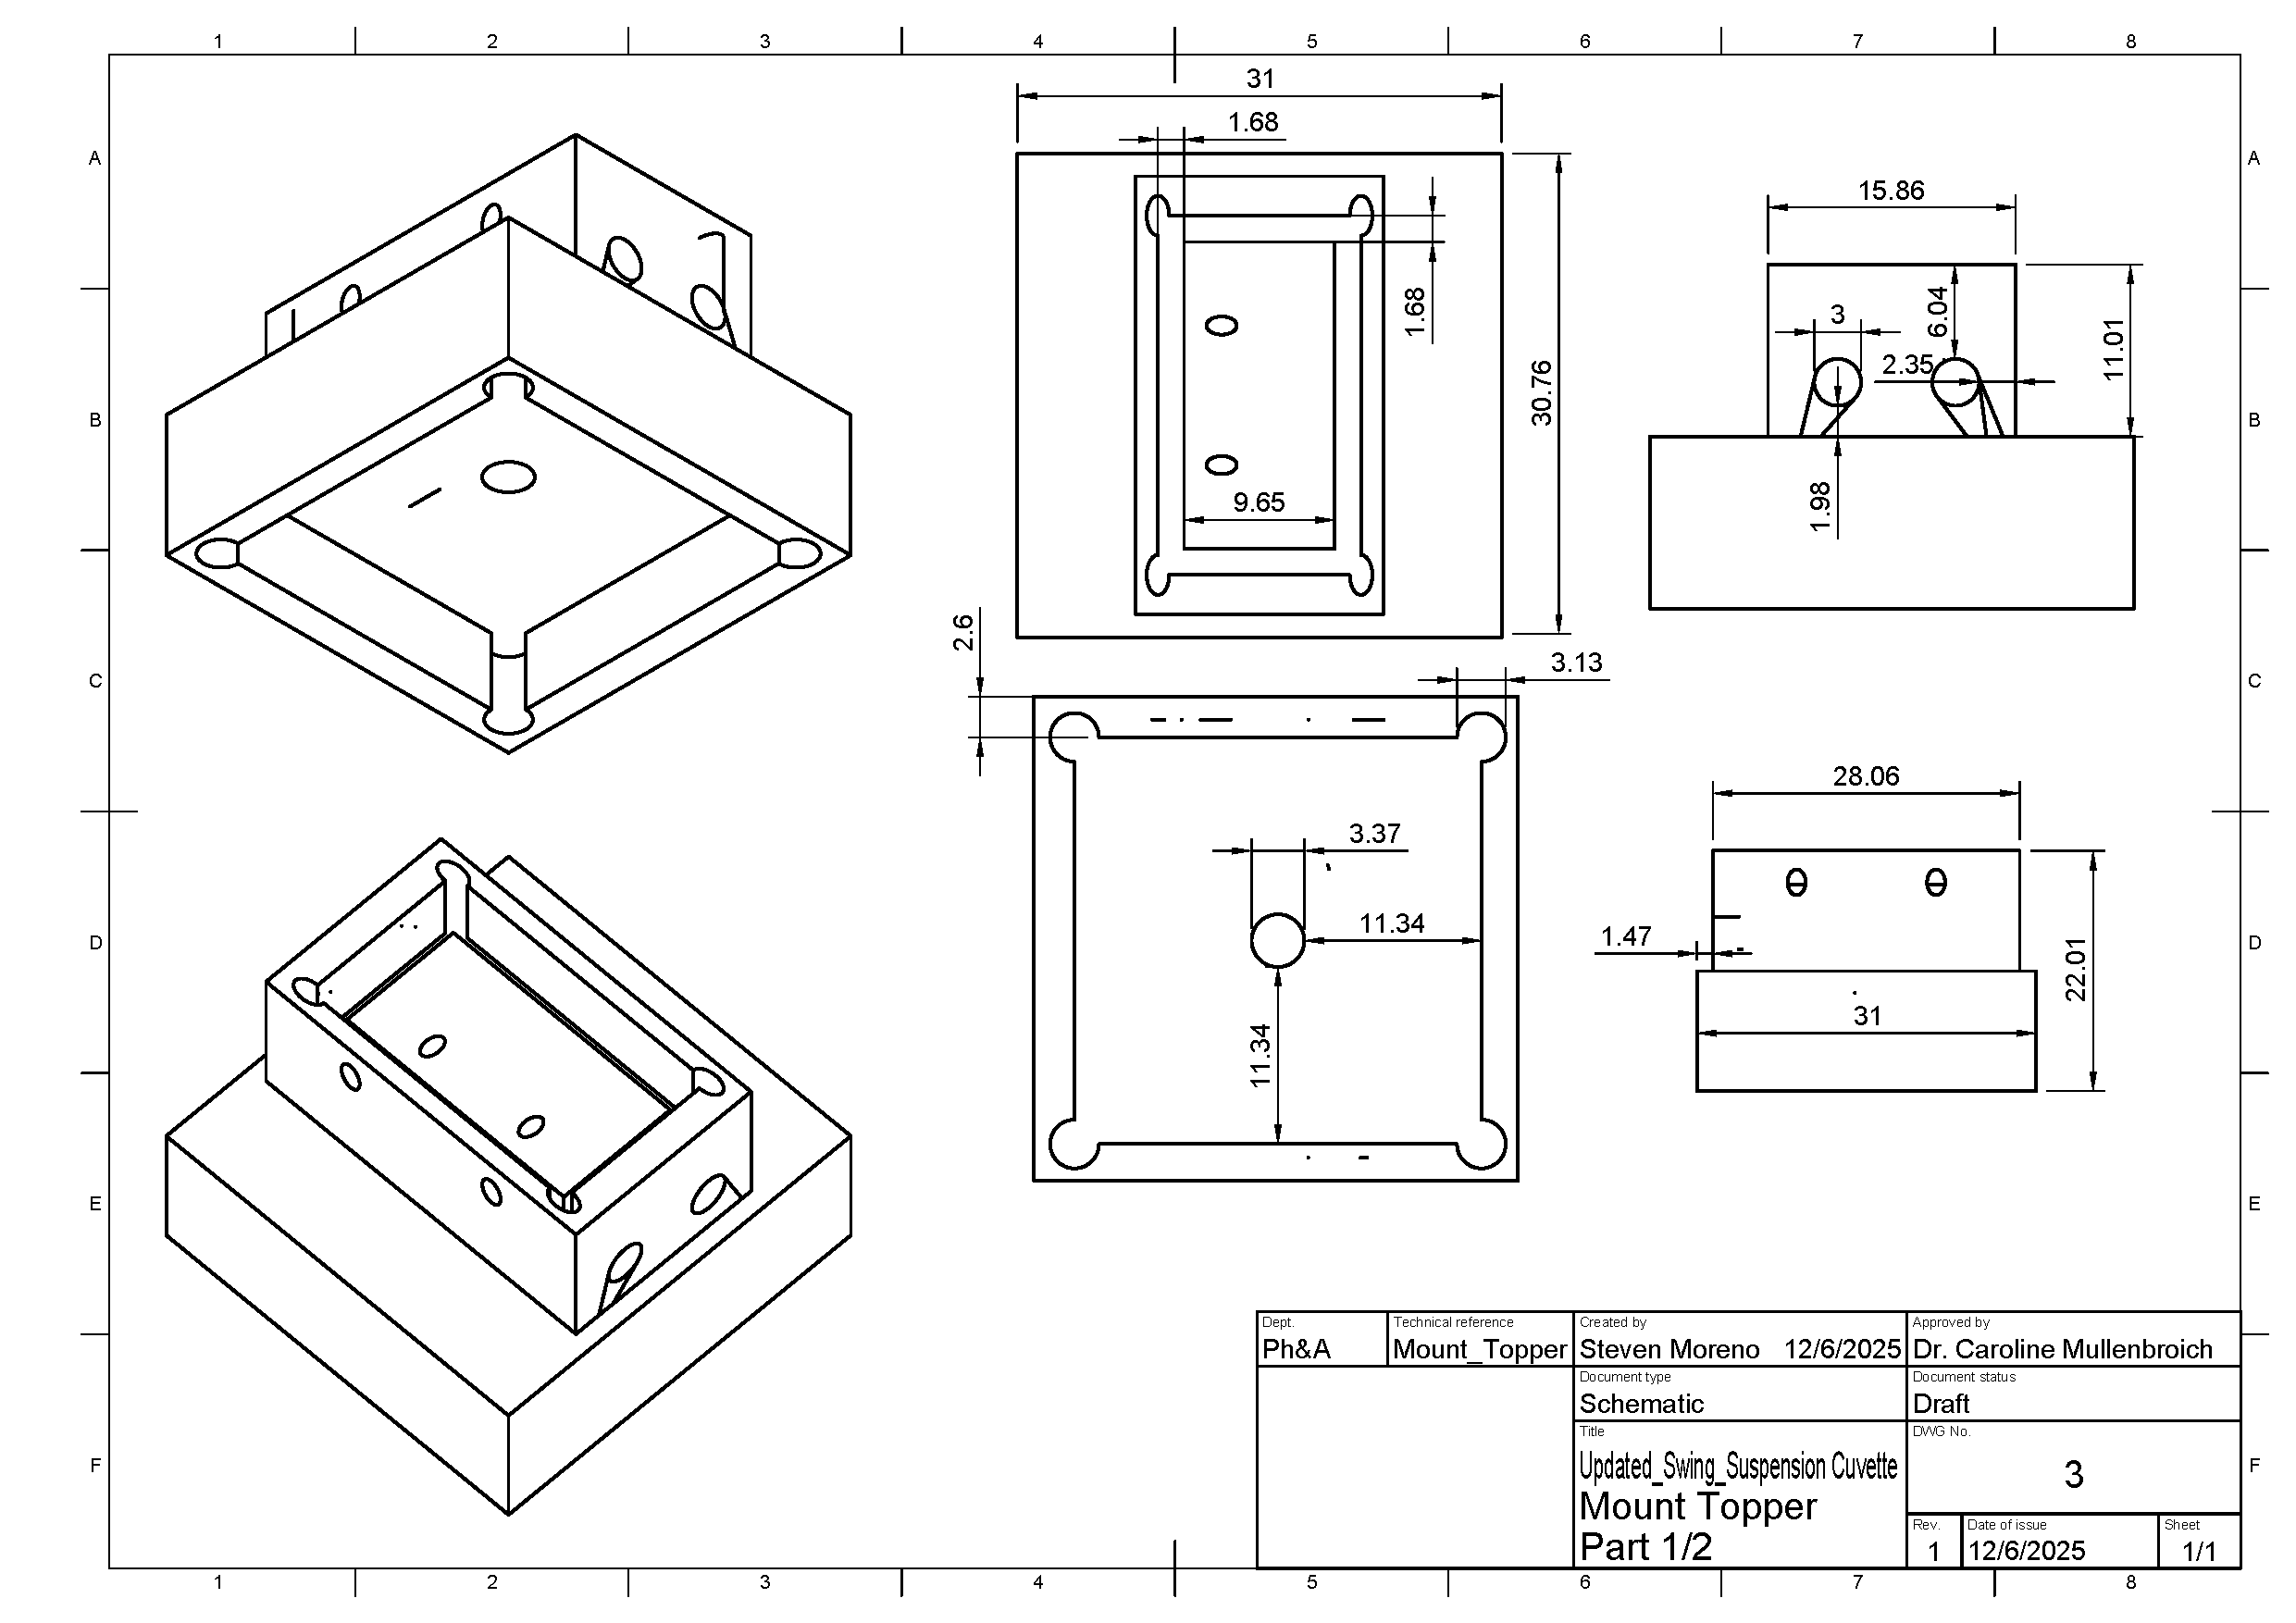
\includegraphics[width=1\linewidth]{Figures/Updated_Swing_Suspension Cuvette Topper Drawing v1.pdf}
    \caption{Schematic of inner cuvette mount topper}
    \end{subfigure}
    \medskip
    
    \begin{subfigure}[c]{0.6\textwidth}
    \centering
    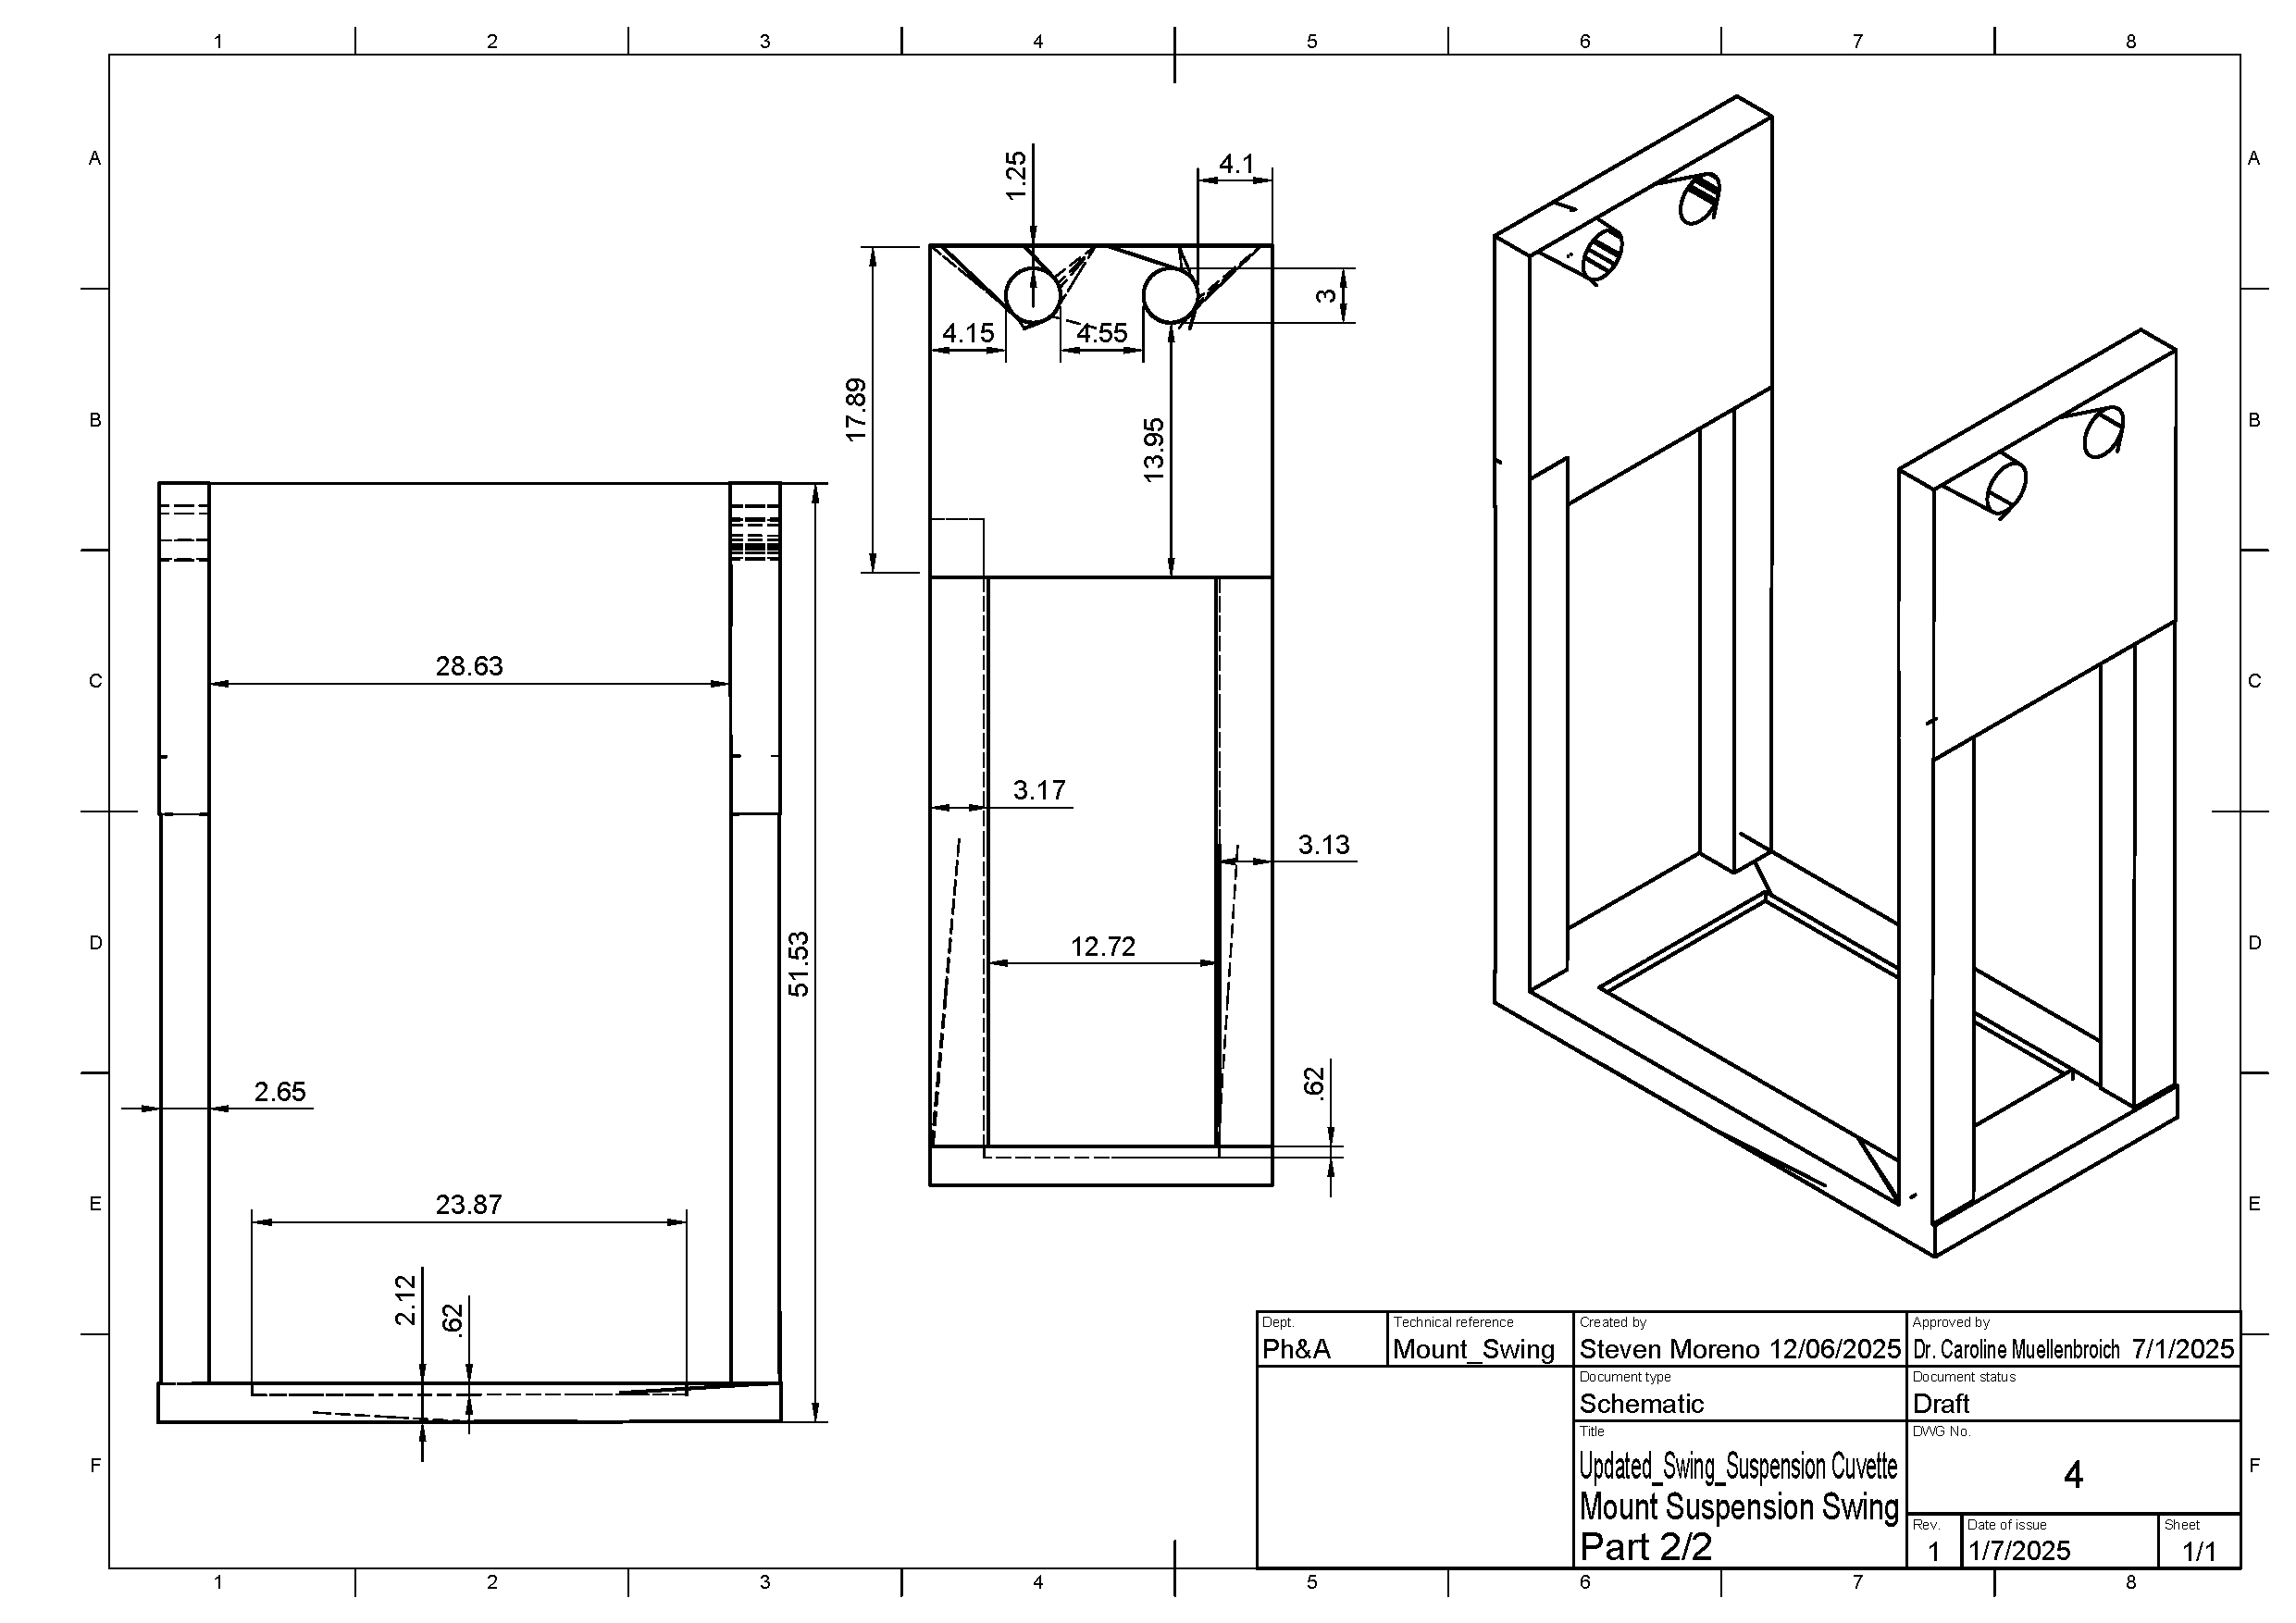
\includegraphics[width=1\linewidth]{Figures/Updated_Swing_Suspension Cuvette Swing v1.pdf}
    \caption{Schematic of mount suspension harness}
    \end{subfigure}
    \medskip

    \begin{subfigure}[d]{1\textwidth}
    \centering
    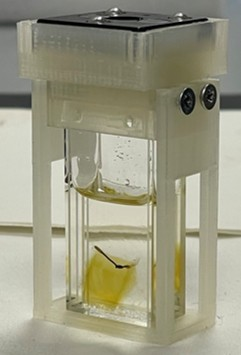
\includegraphics[width=0.25\linewidth]{Images/AssembledMountCUBIC.jpg}
    \caption{\textbf{Fully assembled inner cuvette suspension mount containing cardiac sample and CUBIC-RA solution.}}
    \label{fig:enter-label}
    \end{subfigure}

    \caption{\textbf{Final custom internal cuvette mount and attached suspension platform design for use in mesoSPIM microscope.} Schematics to scale, available in Appendix A.}
\end{figure}


\subsubsection{\textit{Left Ventricle Inner Cuvette Mounting}}

CUBIC-L cleared Left Ventricle samples are placed gently into an optical glass cuvette (Portmann Instruments, UG-205 with the epicardium and endocardium facing the longer sides of the cuvette. The internal volume of the cuvette is then filled to two-thirds full of CUBIC-RA solution. 

The custom designed 3D printed mount holder is then inserted onto the top of the solution filled cuvette. A set of 4 screws (2.5M) are then installed into the bore holes located at the top of suspension platform on opposite sides of the cuvette. These bore holes have corresponding screw bores located on the mount holder that connects the components together. Once installed, the suspension platform holds the cuvette in position with minimal risk of slipping or detaching from the holder. Details and schematics of the inner cuvette holder and suspension platform can be found in Appendix A. 

Once the mount and platform are attached and secured, the sample is left to Refractive Index match to the solution for 10-14 days at room temperature. The sample is concealed from light sources for the duration of this period and is secured in place using soft foam to prevent movement without risking scratching the cuvette walls. RI matching is determined to be complete once the opacity homogenizes and colouration changes from orange to pale yellow colour throughout. Tissues nearing the end of homogenization will also lose any buoyancy in the solution seen at the start of immersion. An example of this completion of RI matching compared to the start of CUBIC-RA immersion can be seen in the figure below:

\begin{figure}[H]
    \centering
    \begin{subfigure}[t]{0.5\textwidth}
        \centering
        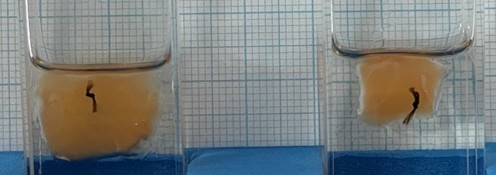
\includegraphics[width=0.8\linewidth]{Images/PreRA.jpg}
        \caption{Start of CUBIC-RA immersion (day 0)}
    \end{subfigure}%
    ~ 
    \begin{subfigure}[t]{0.5\textwidth}
        \centering
        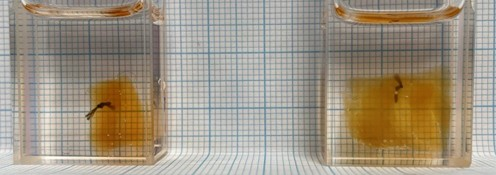
\includegraphics[width=0.8\linewidth]{Images/PostRA.jpg}
        \caption{End of CUBIC-RA immersion (day 14)}
    \end{subfigure}
    \caption{\textbf{CUBIC-RA refractive index matching of LV samples in glass cuvette at start (a) and end (b) of immersion period}. $1mm^2$ grid paper background for scale.}
\end{figure}

\section{Mounted Sample Imaging Characterization}

To quantify and compare the imaging capabilities of the mesoSPIM system to other, more established microscopy methods, a measurement of samples of known dimension and structure would have to be made and recorded using the system. The ability of the system to successfully discern and accurately measure these samples under conditions experienced by tissue samples when mounted inside the system is essential to validate the microscopy techniques used in the imaging pipeline presented here. As such, fluorescent labelled micro-spheres embedded in agarose are utilized to demonstrate the accuracy of the system in recording micron-scale structural targets. This test will also confirm the proper assembly and alignment of the mesoSPIM system  by being able to replicate spatial resolution limits previously reported in other publications using more traditional inner cuvette mounting methods \cite{voigt_mesospim_2019}. These inner cuvette agarose bead samples can also be used to compare the differences in system characterizations between the CLARITY and CUBIC-L/RA protocols as well as serving as a baseline to which alterations to the imaging, mounting protocol can be compared against.

The main alterations to the imaging protocol made in the development of the imaging pipeline were done to de-skew the images captured from oblique positioned sliced samples (see chapter 2, Section 3.2). Alterations to the imaging and processing protocols will allow samples to be digitally reconstructed to appear as they would have if they were imaged at a non-oblique angle, which is required for proper histological analysis to be performed. The ability of these custom protocols were validated by comparing the control characterization of micro-spheres embedded in agar mounted using a traditional cuvette to those mounted using the custom 3D printed mounts. These custom mounted agarose micro-bead samples were, in turn, characterized with shear and no shear techniques to determine how well mechanical de-skewing protocols are able to replicate non-oblique oriented mounting when processed. 


\subsection{Fluorescent Micro-spheres in 1\% Agarose Sample Fabrication} 

\subsubsection{\textit{Agarose Samples in Custom 3D Printed Spacers}}

Two quartz slides are cleaned thoroughly using lens cleaning tissues and then promptly inserted into the custom made, cleared tissue 3D printed mount. Once slotted into place, Eco-Sil Speed Addition Curing Silicone (Picodent®, PIC. 13001000), is thoroughly mixed before then being injected onto the edges of the mount viewing window, ensuring a watertight seal is formed. One side of the mount is fully sealed and left to dry for 20-25 minutes at room temperature. This step is then repeated on the opposite side and left to dry. 

Once the epoxy is fully dry on both sides of the mount, 1\% agarose in deionized $H_2O$ solution is prepared in a sealable microwave safe glass jar by mixing 19.8 mL of deionized $H_2O$ is mixed with 0.2 grams of low gelling temperature agarose (Sigma Aldritch, A9414-25G). The solution is then mixed thoroughly by hand for a minute until the solution is opaque with no large clumps of agarose remaining. The jar lid is then removed and the solution placed into a 800 Watt microwave oven and heated at the medium setting for 60 seconds. The solution is monitored, and the microwave heating is manually stopped once the solution begins to consistently boil. The solution should now be clear in appearance with no clumps or opaque regions visible.

After the solution ceases boiling, the heated jar is carefully removed from the microwave using oven gloves and it is left to cool on the counter-top for 5 minutes. While cooling, 5 uL of 1.04 um Dragon Green fluorescent beads (Bang Laboratories, FSDG004) is measured using a pipette to then be injected into the solution at the end of the cooling period. The jar is sealed closed with the lid and the solution is stirred again for 1 minute by hand. 

After stirring the agarose bead solution, a 0.4 $\mu$m diameter syringe is filled with the liquid solution and injected into the mounts between the slides. The mounts are filled half-way with the bead solution. Once filled, the mount topper is placed on the top of the mounts and the solution is left to cool and gelatinize for 15-20 minutes at room temperature. Once the topper is checked to be firmly in place, a syringe is used to inject EasyIndex\texttrademark\ (EI) Solution (LifeCanvas Technologies, EI-500-1.52) into the remaining empty volume above the agarose gelatin in the mount. A syringe port and air exhaust are built into the topper to allow for simultaneous injection of solution into the mount and expulsion of air out to prevent pressure build ups. Once the mount is filled to the top using EI solution, a lid is inserted over the injection and exhaust ports to prevent dust and debris from entering. The bead sample is then left to immerse in the EI solution for 12-24 hours to permit full perfusion of the solution across the agarose gelatin. Bead samples are then imaged following mounted tissue slice imaging protocols (see chapter 2, section 3).

\subsubsection{\textit{Agarose Samples in Internal Cuvettes}}

For 1\% Agarose Solution Bead Samples to be used in the characterization of the mesoSPIM system using a mounted inner cuvette, the same solution protocol that was documented for samples in 3D printed spacers was followed (See section 2.1 of this chapter). Once the beads are mixed into the solution and sufficiently cooled, the solution is poured into one of two, 7 mL rectangular cuvettes: 1 quartz (Portmann Instruments UQ-205) and 1 optical glass (Portmann Instruments UG-205). Using a plastic 1 mL pipette the bottom third to one-half of the cuvette internal volume is filled (approx.. 2-3.5 mL). The solution is left to cool further and gelatinize for 15-20 minutes. 

After the agarose has set, the cuvette is placed atop a custom designed 3D printed suspension platform. The platform contains a small 1mm deep recess of equal width to the cuvette to ensure secure placement. Once inserted, the remaining internal volume of the optical glass cuvette is filled with CUBIC-RA solution using a plastic pipette and the quartz cuvette is filled with EI solution. Both solutions are added until the meniscus of the solution inside the cuvette is roughly 5mm below the top lip of the cuvette walls (approx. 3.5 mL). 

The custom designed 3D printed mount holder used for left ventricle mounting (see section 1.2 of this chapter) is inserted onto the top of the solution filled cuvette and the remainder of the mounting protocol for this custom mount is followed as previous detailed. The agarose inner cuvette sample proceeds to undergo the inner cuvette imaging protocol previous detailed in chapter 2, section 3. The image stack recorded is set to cover a single tile spanning [GET BEAD STACK DIMENSIONS]. 

\subsection{Customized Image Processing For Oblique Imaging}

With the orientation of the sample being angled at 45 degrees, a method is required to process these images stacks to return them back to a non-oblique orientation. The two methods utilized to achieve this outcome (with and without shearing) will use the following descriptions for axes of orientation: 

\begin{itemize}
    \item At the 0 degree orientation, the sample is parallel to the plane of excitation pathway (x-axis) and perpendicular to the plane of the detection pathway (z-axis) of the mesoSPIM. This will be referred to as the 'system coordinate system' and will be defined here on out as: (\textit{x,z}). 
 
 \item At an 45 degree orientation, the x and z planes of the sample are now translated 45 degrees counter-clockwise from the x,z planes of the system coordinate system. These new axes of orientation will be referred to as the 'sample coordinate system' and will be defined here on out as: (\textit{x',z'}).
\end{itemize}

Python scripts utilized to perform the following oblique image processing techniques can be found in the following Githup repository: [GITHUB URL HERE].

 
\subsubsection{\textit{Sheared Volume Reconstruction}}

A diagram detailing the sheared process of volume reconstruction is shown in Figure 4.6. This sheared method has been previously implemented for use in LSM systems such as OPM and iSPIM and has been modified for use here in the mesoSPIM \cite{wu_inverted_2011, dunsby_optically_2008}. 

\begin{figure}[H]
    \centering
    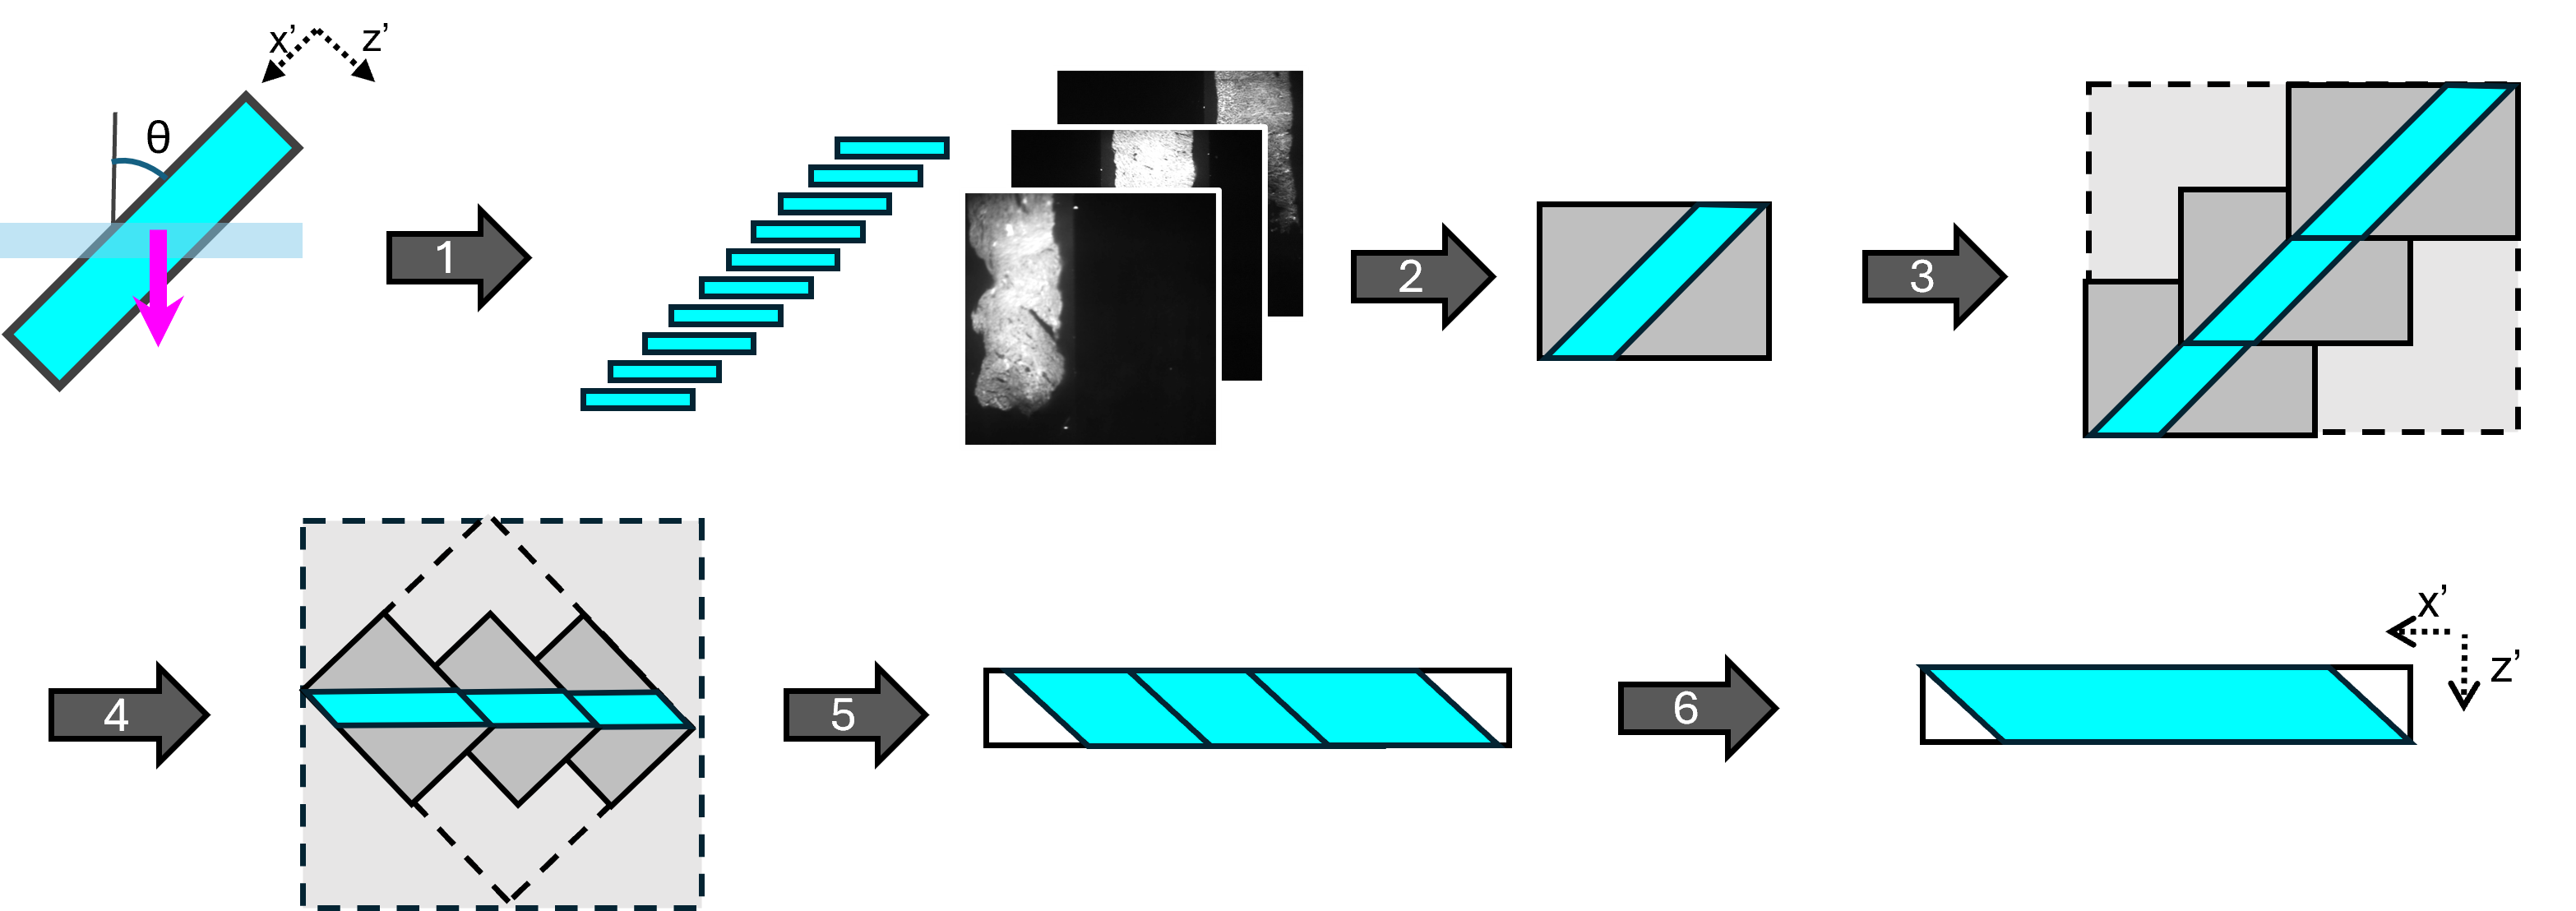
\includegraphics[width=1\linewidth]{Figures/shear.png}
    \medskip
    \caption{\textbf{Sheared scanning of oblique oriented sample for volume reconstruction [].} Diagram legend: Image stack regions occupied by sample volume (cyan); Image stack regions occupied by empty pixels (gray), additional empty pixels added in processing (light gray). Direction of sample movement in the system (magenta arrow) indicated with respect to the system coordinate system.}
    \label{fig:enter-label}
\end{figure}

In this method, as the oblique sample is shifted in z-axis of the system coordinate system, the resulting image series will be sheared as the sample is seen to shift across the camera field of view (Figure 4.6(1-2)) with large blank spaces, void of any signal, found on either side of the sample in every tile and in the stitched image once tiles are combined (4.6(2-3)). These empty regions are an unavoidable consequence of the oblique orientation as only a cross-section of the sample is seen in each frame of the imaging stack. Once acquired, the sheared stack undergoes affine transformation which rotates and scales the data from each frame in the stack, mapping each pixel from the system coordinate system into the sample coordinate system. This process requires the addition of even more regions of empty pixel data to allow digital reorientation of the image stack to occur (Figure 4.6(4-5)). Once reoriented, the sample is reconstructed remaining sheared in the x' and z' axes (Figure 4.6(6)).


\subsubsection{\textit{No-Shear Volume Reconstruction}}

A diagram detailing the no shear process of volume reconstruction is shown in Figure 4.6. This no-sheared method was created during the course of this project in collaboration with primary advisor Dr.Caroline Muellbroich and research colleagues Dr. Sharika Mohanan, Dr. Erin Boland, and Mr. Ahmed Elnageh [CITE OUR PAPER]. 

\begin{figure}[H]
    \centering
    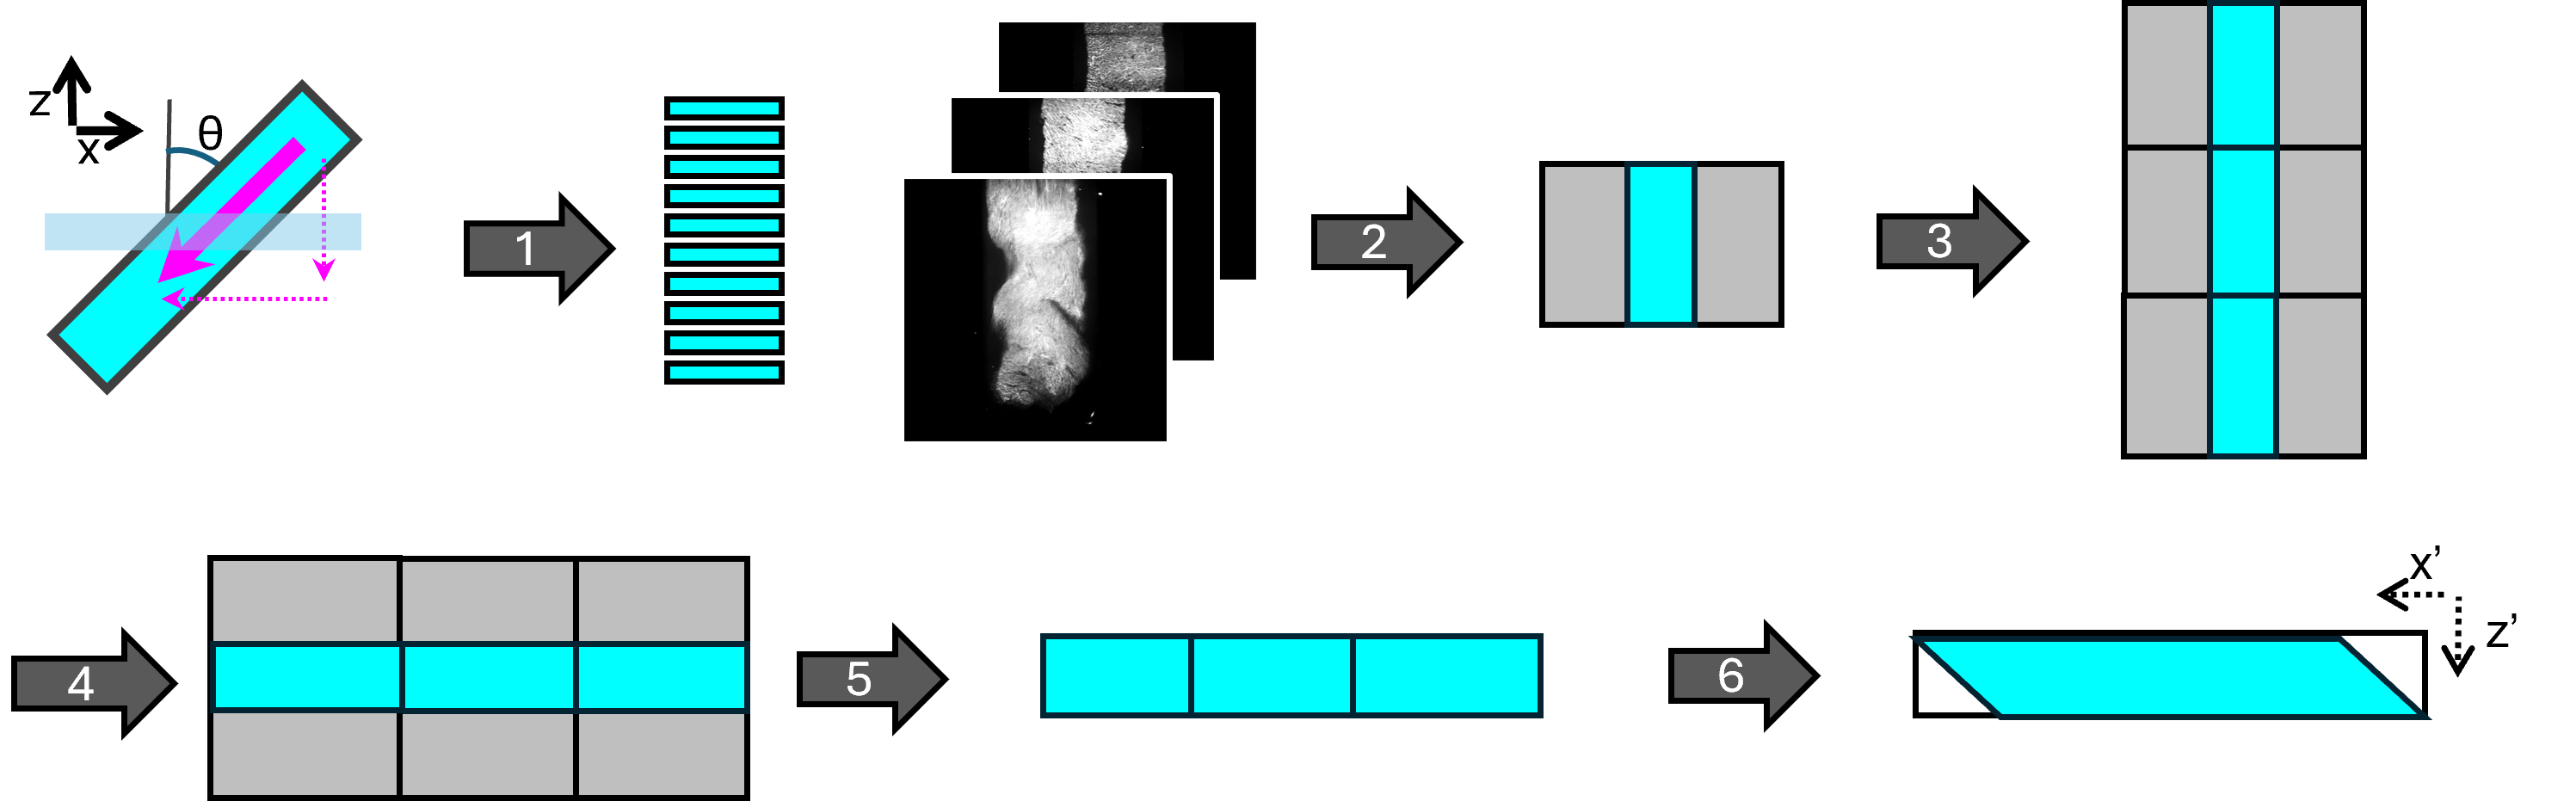
\includegraphics[width=1\linewidth]{Figures/noshear.png}
    \medskip
    \caption{\textbf{No shear scanning of oblique oriented sample for volume reconstruction [].} Diagram legend: Image stack regions occupied by sample (cyan), Image stack regions occupied by empty pixels (gray). Direction of sample movement in the system (magenta arrow) indicated with respect to the system coordinate system.}
    \label{fig:enter-label}
\end{figure}

 The no shear methods activates the x and z axis stages to shift the sample in both axes simultaneously in equal measure between each image captured by the system (Figure 4.7(1)). This movement is in line with the 45 degree orientation of the sample, which shifts the sample to the right in equal amount to shift in the z-axis (Tan 45\degree = 1/1). By shifting the sample in both x and z , the region of the camera FOV occupied by the sample remains unchanged across the entire image stack. To further enhance the axial resolution, the distance traversed by the ETL across the camera FOV during axial scanning protocol is programmed to instead now only span the narrow central region occupied by the tissue []. By decreasing the span of the viable beam region, the central width of the beam is able to be narrowed even further than what is normally achievable using traditional cuvettes, theoretically allowing for even higher resolution than possible when imaging using standard mesoSPIM operation techniques.
 
 Once fully acquired, the Non-sheared Data Stacks are stitched together, rotated 90 degrees, and cropped to isolate the sample from empty pixel regions (Figure 4.7(3-5)). As the sample volume pixels are consistently located in the same region in all frames, the camera FOV regions crop settings are identical in size and position in all frames, expediting the process. Once cropped, the data is scaled on x' axis using affine transform, leaving only the z' axis sheared.

\subsection{Agarose Bead Sample Characterization Results}

Analysis of all Agarose bead samples utilized point spread analysis programs created and optimized by Mr. Ahmed Elnageh in python script [CITE OUR PAPER]. Coding scripts are available in [GITHUB URL, folder location]

\subsubsection{\textit{CLARITY Mount Results}}
\paragraph{Mounted Inner Cuvette}
To provide a control data set to compare data obtained using the custom designed mounts, the spatial resolution of the mesoSPIM using established protocols and mounting methods such as an internal quartz cuvette were recorded and analysed using point spread analysis techniques. The results of this analysis are shown in the following figure.

\begin{figure}[H]
    \centering
     \begin{tikzpicture}
            \begin{axis}
            [
            scale = 1,
            xmin = 1.5,
            xmax = 8.5,
            ylabel={Spatial Axis},
            xlabel={Recorded Measurement (microns)},
            ytick={1,2,3},
            yticklabels={Z,Y,X}, 
            boxplot/box extend=0.25,
            ]
    
    \addplot+ [boxplot] 
            table [y index=0] {Data/rect_cuvette/zfwhm.txt}
            [above]
            node at
              (boxplot whisker cs:\boxplotvalue{lower whisker},1)
              {\pgfmathprintnumber{\boxplotvalue{lower whisker}}}
            node at
              (boxplot box cs: \boxplotvalue{median},1)
              {\pgfmathprintnumber{\boxplotvalue{median}}}
            node at
              (boxplot whisker cs:\boxplotvalue{upper whisker},1)
              {\pgfmathprintnumber{\boxplotvalue{upper whisker}}}
            ;
            
    \addplot+[boxplot] 
            table [y index=0] {Data/rect_cuvette/yfwhm.txt}
            [above]
            node at
              (boxplot whisker cs:\boxplotvalue{lower whisker},1)
              {\pgfmathprintnumber{\boxplotvalue{lower whisker}}}
            node at
              (boxplot box cs: \boxplotvalue{median},-1)
              {\pgfmathprintnumber{\boxplotvalue{median}}}
            node at
              (boxplot whisker cs:\boxplotvalue{upper whisker},1)
              {\pgfmathprintnumber{\boxplotvalue{upper whisker}}}
            ;
            
    \addplot+[boxplot] 
            table [y index=0] {Data/rect_cuvette/xfwhm.txt}
            [above]
            node at
              (boxplot whisker cs:\boxplotvalue{lower whisker},1)
              {\pgfmathprintnumber{\boxplotvalue{lower whisker}}}
            node at
              (boxplot box cs: \boxplotvalue{median},-1)
              {\pgfmathprintnumber{\boxplotvalue{median}}}
            node at
              (boxplot whisker cs:\boxplotvalue{upper whisker},1)
              {\pgfmathprintnumber{\boxplotvalue{upper whisker}}}
            ;
                       
            \end{axis}
        \end{tikzpicture}
    \caption{\textbf{[ADD UNITS]Point spread analysis: Quartz glass cuvette, florescent beads in agarose solution} Box plots of full width at half maximum (FWHM) of 1 micron florescent beads dimensions measured in recording (n = 1278 beads).}
    \label{fig:enter-label}
\end{figure}


The average FWHM of the recorded sub-resolution beads in the x,y, and z axes were calculated to be 3.95$\pm$0.8 microns, 5.22$\pm$1.06 microns, and 5.96$\pm$0.75 microns respectively [DOUBLE CHECK]. This data is suggests the system has poorer resolution compared to other assembled mesoSPIM systems \cite{voigt_mesospim_2019}. This was expected due to the deactivation of one excitation in the mesoSPIM, difficulties in properly aligning the system, as well as the potential mismatch of the RIMS aqueous solution mediums used which may have not been sufficiently mixed or experienced gradual evaporation of water in the solution over time, altering the RI.

\paragraph{Sheared Vs No Shear}
Next, the spatial resolution of the mesoSPIM using the new custom made mounts in combination with shear and no shear protocols were recorded and analysed using point spread analysis techniques. Both protocols were performed using 4 separate agarose solution filled mounts to ensure the results acquired using the custom designed mounts are repeatable with minimal differences in achievable resolution between each mount. The results of the no shear recordings were collected and are compared side by side in Figure 4.9 (a-d):

\begin{figure}[H]
\centering
    \begin{subfigure}[t]{0.46\textwidth}
        \centering
        \begin{tikzpicture}
            \begin{axis}
            [
            scale = 0.9,
            xmin = 2,
            xmax = 13,
            ytick={1,2,3},
            yticklabels={Z',Y, X'}, 
            ylabel={Spatial Axis},
            xlabel={Recorded Measurement (microns)},
            boxplot/box extend=0.25,
            ]
    
    \addplot+ [boxplot] 
            table [y index=0] {Data/B4_2/2zfwhm.txt}
            [above]
            node at
              (boxplot whisker cs:\boxplotvalue{lower whisker},1)
              {\pgfmathprintnumber{\boxplotvalue{lower whisker}}}
            node at
              (boxplot box cs: \boxplotvalue{median},1)
              {\pgfmathprintnumber{\boxplotvalue{median}}}
            node at
              (boxplot whisker cs:\boxplotvalue{upper whisker},1)
              {\pgfmathprintnumber{\boxplotvalue{upper whisker}}}
            ;
            
    \addplot+[boxplot] 
            table [y index=0] {Data/B4_2/2yfwhm.txt}
            [above]
            node at
              (boxplot whisker cs:\boxplotvalue{lower whisker},1)
              {\pgfmathprintnumber{\boxplotvalue{lower whisker}}}
            node at
              (boxplot box cs: \boxplotvalue{median},-1)
              {\pgfmathprintnumber{\boxplotvalue{median}}}
            node at
              (boxplot whisker cs:\boxplotvalue{upper whisker},1)
              {\pgfmathprintnumber{\boxplotvalue{upper whisker}}}
            ;
            
    \addplot+[boxplot] 
            table [y index=0] {Data/B4_2/2xfwhm.txt}
            [above]
            node at
              (boxplot whisker cs:\boxplotvalue{lower whisker},1)
              {\pgfmathprintnumber{\boxplotvalue{lower whisker}}}
            node at
              (boxplot box cs: \boxplotvalue{median},-1)
              {\pgfmathprintnumber{\boxplotvalue{median}}}
            node at
              (boxplot whisker cs:\boxplotvalue{upper whisker},1)
              {\pgfmathprintnumber{\boxplotvalue{upper whisker}}}
            ;
                       
            \end{axis}
        \end{tikzpicture}
        \caption{\textbf{Agarose Bead Mount \#1 (n = 1185)}}
    \end{subfigure}
    \medskip
    \hspace{1em}
    ~
    \begin{subfigure}[t]{0.46\textwidth}
        \centering
        \begin{tikzpicture}
             \begin{axis}
            [
            scale = 0.9,
            xmin = 2,
            xmax = 13,
            ytick={1,2,3},
            yticklabels={Z',Y, X'},
            ylabel={Spatial Axis},
            xlabel={Recorded Measurement (microns)},
            boxplot/box extend=0.25,
            ]
    
    \addplot+ [boxplot] 
            table [y index=0] {Data/B4_3/3zfwhm.txt}
            [above]
            node at
              (boxplot whisker cs:\boxplotvalue{lower whisker},1)
              {\pgfmathprintnumber{\boxplotvalue{lower whisker}}}
            node at
              (boxplot box cs: \boxplotvalue{median},-1)
              {\pgfmathprintnumber{\boxplotvalue{median}}}
            node at
              (boxplot whisker cs:\boxplotvalue{upper whisker},1)
              {\pgfmathprintnumber{\boxplotvalue{upper whisker}}}
            ;
            
    \addplot+[boxplot] 
            table [y index=0] {Data/B4_3/3yfwhm.txt}
            [above]
            node at
              (boxplot whisker cs:\boxplotvalue{lower whisker},1)
              {\pgfmathprintnumber{\boxplotvalue{lower whisker}}}
            node at
              (boxplot box cs: \boxplotvalue{median},1)
              {\pgfmathprintnumber{\boxplotvalue{median}}}
            node at
              (boxplot whisker cs:\boxplotvalue{upper whisker},1)
              {\pgfmathprintnumber{\boxplotvalue{upper whisker}}}
            ;
            
    \addplot+[boxplot] 
            table [y index=0] {Data/B4_3/3xfwhm.txt}
            [above]
            node at
              (boxplot whisker cs:\boxplotvalue{lower whisker},1)
              {\pgfmathprintnumber{\boxplotvalue{lower whisker}}}
            node at
              (boxplot box cs: \boxplotvalue{median},-1)
              {\pgfmathprintnumber{\boxplotvalue{median}}}
            node at
              (boxplot whisker cs:\boxplotvalue{upper whisker},1)
              {\pgfmathprintnumber{\boxplotvalue{upper whisker}}}
            ;
            [
                       
            \end{axis}
        \end{tikzpicture}
        \caption{\textbf{Agarose Bead Mount \#2 (n = 407)}}
    \end{subfigure}
    \medskip
    
\begin{subfigure}[t]{0.46\textwidth}
        \centering
        \begin{tikzpicture}
            \begin{axis}
            [
            scale = 0.9,
            xmin = 2,
            xmax = 13,
            ytick={1,2,3},
            yticklabels={Z',Y, X'},
            ylabel={Spatial Axis},
            xlabel={Recorded Measurement (microns)},
            boxplot/box extend=0.25,
            ]
    
    \addplot+ [boxplot] 
            table [y index=0] {Data/B4_4/4zfwhm.txt}
            [above]
            node at
              (boxplot whisker cs:\boxplotvalue{lower whisker},1)
              {\pgfmathprintnumber{\boxplotvalue{lower whisker}}}
            node at
              (boxplot box cs: \boxplotvalue{median},1)
              {\pgfmathprintnumber{\boxplotvalue{median}}}
            node at
              (boxplot whisker cs:\boxplotvalue{upper whisker},1)
              {\pgfmathprintnumber{\boxplotvalue{upper whisker}}}
            ;
            
    \addplot+[boxplot] 
            table [y index=0] {Data/B4_4/4yfwhm.txt}
            [above]
            node at
              (boxplot whisker cs:\boxplotvalue{lower whisker},1)
              {\pgfmathprintnumber{\boxplotvalue{lower whisker}}}
            node at
              (boxplot box cs: \boxplotvalue{median},-1)
              {\pgfmathprintnumber{\boxplotvalue{median}}}
            node at
              (boxplot whisker cs:\boxplotvalue{upper whisker},1)
              {\pgfmathprintnumber{\boxplotvalue{upper whisker}}}
            ;
            
    \addplot+[boxplot] 
            table [y index=0] {Data/B4_4/4xfwhm.txt}
            [above]
            node at
              (boxplot whisker cs:\boxplotvalue{lower whisker},1)
              {\pgfmathprintnumber{\boxplotvalue{lower whisker}}}
            node at
              (boxplot box cs: \boxplotvalue{median},-1)
              {\pgfmathprintnumber{\boxplotvalue{median}}}
            node at
              (boxplot whisker cs:\boxplotvalue{upper whisker},1)
              {\pgfmathprintnumber{\boxplotvalue{upper whisker}}}
            ;
            [
                       
            \end{axis}
        \end{tikzpicture}
        \caption{\textbf{Agarose Bead Mount \#3 (n = 1341)}}
    \end{subfigure}
    \medskip
    \hspace{1em}
    ~
    \begin{subfigure}[t]{0.46\textwidth}
        \centering
        \begin{tikzpicture}
             \begin{axis}
             [
            scale = 0.9,
            xmin = 2,
            xmax = 13,
            ytick={1,2,3},
            yticklabels={Z',Y, X'},
            ylabel={Spatial Axis},
            xlabel={Recorded Measurement (microns)},
            boxplot/box extend=0.25,
            ]
    
    \addplot+ [boxplot] 
            table [y index=0] {Data/B4_5/5zfwhm.txt}
            [above]
            node at
              (boxplot whisker cs:\boxplotvalue{lower whisker},1)
              {\pgfmathprintnumber{\boxplotvalue{lower whisker}}}
            node at
              (boxplot box cs: \boxplotvalue{median},-1)
              {\pgfmathprintnumber{\boxplotvalue{median}}}
            node at
              (boxplot whisker cs:\boxplotvalue{upper whisker},1)
              {\pgfmathprintnumber{\boxplotvalue{upper whisker}}}
            ;
            
    \addplot+[boxplot] 
            table [y index=0] {Data/B4_5/5yfwhm.txt}
            [above]
            node at
              (boxplot whisker cs:\boxplotvalue{lower whisker},1)
              {\pgfmathprintnumber{\boxplotvalue{lower whisker}}}
            node at
              (boxplot box cs: \boxplotvalue{median},1)
              {\pgfmathprintnumber{\boxplotvalue{median}}}
            node at
              (boxplot whisker cs:\boxplotvalue{upper whisker},1)
              {\pgfmathprintnumber{\boxplotvalue{upper whisker}}}
            ;
            
    \addplot+[boxplot] 
            table [y index=0] {Data/B4_5/5xfwhm.txt}
            [above]
            node at
              (boxplot whisker cs:\boxplotvalue{lower whisker},1)
              {\pgfmathprintnumber{\boxplotvalue{lower whisker}}}
            node at
              (boxplot box cs: \boxplotvalue{median},-1)
              {\pgfmathprintnumber{\boxplotvalue{median}}}
            node at
              (boxplot whisker cs:\boxplotvalue{upper whisker},1)
              {\pgfmathprintnumber{\boxplotvalue{upper whisker}}}
            ;
            [
                       
            \end{axis}
        \end{tikzpicture}
        \caption{\textbf{Agarose Bead Mount \#4 (n = 761)}}
    \end{subfigure}
    \caption{\textbf{Agarose bead samples point spread analysis: 4 Custom 3D Printed Mounts, No Shear Technique} Box plots of full width at half maximum (FWHM) results in x',y, and z' sample coordinate axes. Median, upper and lower quartiles, max and min extrema shown (N,overall = 3691 beads)}
    \label{fig:enter-label}
\end{figure}

 The average FWHM results of sheared and no sheared recordings taken of the same agarose bead sample set are compared side by side in Figure 4.10.

\begin{figure}[H] 
    \centering
    \begin{subfigure}[t]{0.46\textwidth}
    \centering
        \begin{tikzpicture}
            \begin{axis}
             [
            scale = 0.9,
            xmin = 2,
            xmax = 15.5,
            ytick={1,2,3},
            yticklabels={Z',Y, X'},
            ylabel={Spatial Axis},
            xlabel={Recorded Measurement (microns)},
            boxplot/box extend=0.25,
            ]

            \addplot+ [boxplot] 
                    table [y index=0] {Data/double/zfwhm.txt}
                    [above]
                    node at
                      (boxplot whisker cs:\boxplotvalue{lower whisker},1)
                      {\pgfmathprintnumber{\boxplotvalue{lower whisker}}}
                    node at
                      (boxplot box cs: \boxplotvalue{median},-1)
                      {\pgfmathprintnumber{\boxplotvalue{median}}}
                    node at
                      (boxplot whisker cs:\boxplotvalue{upper whisker},1)
                      {\pgfmathprintnumber{\boxplotvalue{upper whisker}}}
                    ;
                    
            \addplot+[boxplot] 
                    table [y index=0] {Data/double/yfwhm.txt}
                    [above]
                    node at
                      (boxplot whisker cs:\boxplotvalue{lower whisker},1)
                      {\pgfmathprintnumber{\boxplotvalue{lower whisker}}}
                    node at
                      (boxplot box cs: \boxplotvalue{median},1)
                      {\pgfmathprintnumber{\boxplotvalue{median}}}
                    node at
                      (boxplot whisker cs:\boxplotvalue{upper whisker},1)
                      {\pgfmathprintnumber{\boxplotvalue{upper whisker}}}
                    ;
                    
            \addplot+[boxplot] 
                    table [y index=0] {Data/double/xfwhm.txt}
                    [above]
                    node at
                      (boxplot whisker cs:\boxplotvalue{lower whisker},1)
                      {\pgfmathprintnumber{\boxplotvalue{lower whisker}}}
                    node at
                      (boxplot box cs: \boxplotvalue{median},-1)
                      {\pgfmathprintnumber{\boxplotvalue{median}}}
                    node at
                      (boxplot whisker cs:\boxplotvalue{upper whisker},1)
                      {\pgfmathprintnumber{\boxplotvalue{upper whisker}}}
                    ;
            [
                       
            \end{axis}
        \end{tikzpicture}
    \caption{\textbf{Averaged point spread analysis: Custom 3D printed mount, shear technique} Box plots of average FWHM in examined agarose bead samples (m = 4).}
    \end{subfigure}
    \hspace{2em}
    ~
    \begin{subfigure}[t]{0.46\textwidth}
        \centering
            \begin{tikzpicture}
                 \begin{axis}
                 [
                scale = 0.9,
                xmin = 2,
                xmax = 15.5,
                ytick={1,2,3},
                yticklabels={Z',Y, X'},
                ylabel={Spatial Axis},
                xlabel={Recorded Measurement (microns)},
                boxplot/box extend=0.25,
                ]
        
        \addplot+ [boxplot] 
                table [y index=0] {Data/double/nzfwhm.txt}
                [above]
                node at
                  (boxplot whisker cs:\boxplotvalue{lower whisker},1)
                  {\pgfmathprintnumber{\boxplotvalue{lower whisker}}}
                node at
                  (boxplot box cs: \boxplotvalue{median},-1)
                  {\pgfmathprintnumber{\boxplotvalue{median}}}
                node at
                  (boxplot whisker cs:\boxplotvalue{upper whisker},1)
                  {\pgfmathprintnumber{\boxplotvalue{upper whisker}}}
                ;
                
        \addplot+[boxplot] 
                table [y index=0] {Data/double/nyfwhm.txt}
                [above]
                node at
                  (boxplot box cs:\boxplotvalue{lower whisker},0.9)
                  {\pgfmathprintnumber{\boxplotvalue{lower whisker}}}
                node at
                  (boxplot box cs: \boxplotvalue{median},-1)
                  {\pgfmathprintnumber{\boxplotvalue{median}}}
                node at
                  (boxplot box cs:\boxplotvalue{upper whisker},1)
                  {\pgfmathprintnumber{\boxplotvalue{upper whisker}}}
                ;
                
        \addplot+[boxplot] 
                table [y index=0] {Data/double/nxfwhm.txt}
                [above]
                node at
                  (boxplot whisker cs:\boxplotvalue{lower whisker},1)
                  {\pgfmathprintnumber{\boxplotvalue{lower whisker}}}
                node at
                  (boxplot box cs: \boxplotvalue{median},-1)
                  {\pgfmathprintnumber{\boxplotvalue{median}}}
                node at
                  (boxplot whisker cs:\boxplotvalue{upper whisker},1)
                  {\pgfmathprintnumber{\boxplotvalue{upper whisker}}}
                ;
                [      
                \end{axis}
            \end{tikzpicture}
    \caption{\textbf{Averaged point spread analysis: Custom 3D printed mount, no shear technique} Box plots of average FWHM in examined agarose bead samples (m = 4).}
    \end{subfigure}

    \label{fig:enter-label}
    \caption{\textbf{Point spread analysis comparison: Shear and no shear techniques.} 1 micron florescent beads in agarose solution dimensions measured in recordings: Shear recording (n = 314 beads); No shear recording (n = 3673 beads).}
\end{figure}

Over the 4 custom mount samples created and recorded using the shear technique, the average FWHM of the recorded sub-resolution beads in the x',y, and z' axes were calculated to be 5.94$\pm$0.77 microns, 8.12$\pm$1.32 microns, and 13.23$\pm$0.72 microns respectively. In comparison, the average FWHM of the same 4 custom mount samples recorded using the no-shear technique were calculated to be 4.66$\pm$0.67 microns in x'-axis, 3.86$\pm$0.49 microns in the y-axis, and 7.76$\pm$1.64 microns in the z'-axis.

Between Shear and No Shear techniques, axial resolution (in the z'-axis) is found to double using the no shear method while lateral resolution is seen to have an approximately 30\% increase in the y-axis. Resolution in the x'-axis was found to be similar in both methods as anticipated with both images remaining sheared in that specific axis. Significant overlap is seen in the calculated error margins of x'-axis resolution, though spread of measurements in the no-shear x'-axis data contained slightly less variation.

To quantify changes in resolution anisotropy between shear and no shear, the anisotropy ratio (A) was determined between the FWHM of the x and y axis components of lateral resolution in both averaged data sets. 

\begin{equation}
A = \frac{FWHM_x}{FWHM_y}
\end{equation}
\medskip

The Anisotropy Ratio in the sheared data was found to be at 1.34 while the ratio was 0.61 in the no shear data, indicating the lateral anisotropy had increased in the no-shear recordings as a result of the reduced FWHM value of the y-axis and generally consistent FWHM value found in the x-axis. 

\subsubsection{\textit{CUBIC-L/RA Inner Cuvette Results}}
The spatial resolution of the mesoSPIM using established CUBIC-L/RA protocols and mounting methods such as an internal optical glass cuvette were recorded and analysed using point spread analysis techniques. The results of this characterization are shown in the following figure.

\begin{figure}[H]
    \centering
     \begin{tikzpicture}
            \begin{axis}
            [
            scale = 1,
            xmin = 1.5,
            xmax = 7.5,
            ytick={1,2,3},
            yticklabels={Z,Y,X}, 
            ylabel={Spatial Axis},
            xlabel={Recorded Measurement (microns)},
            boxplot/box extend=0.25,
            ]
    
    \addplot+ [boxplot] 
            table [y index=0] {Data/cubic_cuvette/488nm/zfwhm.txt}
            [above]
            node at
              (boxplot whisker cs:\boxplotvalue{lower whisker},1)
              {\pgfmathprintnumber{\boxplotvalue{lower whisker}}}
            node at
              (boxplot box cs: \boxplotvalue{median},1)
              {\pgfmathprintnumber{\boxplotvalue{median}}}
            node at
              (boxplot whisker cs:\boxplotvalue{upper whisker},1)
              {\pgfmathprintnumber{\boxplotvalue{upper whisker}}}
            ;
            
    \addplot+[boxplot] 
            table [y index=0] {Data/cubic_cuvette/488nm/yfwhm.txt}
            [above]
            node at
              (boxplot whisker cs:\boxplotvalue{lower whisker},1)
              {\pgfmathprintnumber{\boxplotvalue{lower whisker}}}
            node at
              (boxplot box cs: \boxplotvalue{median},-1)
              {\pgfmathprintnumber{\boxplotvalue{median}}}
            node at
              (boxplot whisker cs:\boxplotvalue{upper whisker},1)
              {\pgfmathprintnumber{\boxplotvalue{upper whisker}}}
            ;
            
    \addplot+[boxplot] 
            table [y index=0] {Data/cubic_cuvette/488nm/xfwhm.txt}
            [above]
            node at
              (boxplot whisker cs:\boxplotvalue{lower whisker},1)
              {\pgfmathprintnumber{\boxplotvalue{lower whisker}}}
            node at
              (boxplot box cs: \boxplotvalue{median},-1)
              {\pgfmathprintnumber{\boxplotvalue{median}}}
            node at
              (boxplot whisker cs:\boxplotvalue{upper whisker},1)
              {\pgfmathprintnumber{\boxplotvalue{upper whisker}}}
            ;
                       
            \end{axis}
        \end{tikzpicture}
    \caption{\textbf{Point spread analysis: Optical glass cuvette, florescent beads in agarose solution} Box plots of full width at half maximum (FWHM) of 1 micron florescent beads examined in recording (n = 1278 beads).}
    \label{fig:enter-label}
\end{figure}

The average FWHM of the recorded sub-resolution beads in the x,y, and z axes were calculated to be 4.19$\pm$0.64 microns, 3.85$\pm$0.42 microns, and 4.61$\pm$1.12 microns respectively in the 488 nm channel. This data is consistent with previous examinations of spatial resolution of the mesoSPIM using similar mounting techniques[]. 

\section{Discussion}
The main aim of this series of experiments was to produce an optimized tissue mounting procedure and data processing methodology to obtain unaltered structural data utilizing these novel, 3D printed mounting designs. The results obtained from the experiments described in this chapter confirms that the finalized pipeline protocols described in Chapter 4.1 is fully capable of producing high quality images of ex vivo tissue structure when implemented as part of the overarching tissue imaging pipeline. 

\subsection{Tissue Mounting Discussion}
\subsubsection{\textit{Sliced Tissue Mounting Discussion}}
In the process of designing mounts for the imaging of CLARITY cleared tissue samples, there was a considerable convenience seen in the fact that the mounting frame required for the clearing process (See Chapter 3.1) could also be utilized for imaging with the addition of 3D components to overlay the base mount. Basic resizing of the mount to allow the insertion of slightly wider (0.1-0.2 mm) and thinner (0.05-0.1 mm) quartz slides instead of standard issue microscope soda-lime glass slides used in the CLARITY protocol was the only change required, with all other requirements for the imaging mount (such as being able to be suspended from the sample gantry using a Thorlabs post holder, allowing for the injection of RI matching solution, and being able to be stored for extended periods of time between imaging session) being met by the addition of a Thorlabs post-holder compatible mount topper with sealable syringe injection ports. The simplicity of the design of all three of these components meant modifications can easily be made to allow samples and slides of various width and thickness to be imaged utilizing this imaging process. 

\subsubsection{\textit{Left Ventricle Mounting Discussion}}

Initial designs which used friction applied by nylon screws onto the cuvette walls to suspend the cuvette from the top were abandoned. This method proved to unreliable and was prone to damaging to the cuvette gradually over time. Preserving the condition of the fragile cuvette walls during imaging was made a priority, ensuring no cracks or scratching occurred while the mount was assembled, in use, and when removed after imaging. In the place of the initial design, a new mount design would instead support the cuvette from below with the new bore holes added to the old mount topper design to attach the bottom support frame.

Another factor taken into consideration for the mount's design was the limited volume the cuvette could safely traverse without coming into contact with the sides or base of the outer cuvette installed into the mesoSPIM system. Supports attached to the cuvette from the bottom of the cuvette would reduce the depth the cuvette could be lowered without impacting the outer cuvette base. This same issue holds true for the support frame that must span across the sides of the inner cuvette to connect the base platform to the mount topper. For these reasons, the attachable base platform created for use with the cuvette mount topper was made as thin and narrow as possible while maintaining its ability to support the inner cuvette from beneath. This allows the cuvette to traverse the largest volume in the outer cuvette possible while also keeping the inner cuvette securely affixed to the sample gantry suspended above the detection path.



\subsection{Imaging Characterization Discussion}
A successful mounting and associated data acquisition process was established for use in the imaging pipeline utilizing CLARITY cleared tissue slices. Shearing and aberrations seen from the oblique imaging methods used to record images of sliced samples contained in custom made mounts were compensated for in the data processing conducted on the raw data after acquisition. The adjustments made to the imaging process further aided in reducing the processing demands required to restore the image back to a non-oblique orientation. By implementing the no-shear protocol (see Figure 4.7), the excessive additions of empty pixel data and the affine transformation performed on multiple axis seen in the shear method (See Figure 4.6) were eliminated. In their place, simple image matrix rotation, rescaling, and affine transformation in just one axis is required, streamlining the processing method and reducing the file size of data sets by up to five times in some cases. 

Results from characterization tests performed confirm the no-shear protocols as superior in acquiring higher image quality compared to sheared methods. The axial resolution achievable by the no-shear technique was even found to be roughly double that of the sheared techniques a result of the reduced ETL range of movement, which could not be easily replicated in sheared imaging without significant alteration to the mesoSPIM software.

The recorded z-axis resolutions obtained in these experiments establishes the 2 and 3 microns step sizes to be implemented when recording image stacks of tissue samples using these mounting and image processing techniques. These z-steps signify the distance between each frame recorded by the mesoSPIM and is set to be roughly 50\% of the axial FWHM distance determined for each mounting method, ensuring sufficient sampling of tissue volume is collected during imaging sessions. 


\subsubsection{\textit{Aberration Induced Variability In Mounted Sliced Tissue Characterization}}

The results seen from no-shear characterization were reasonably similar to the resolution and image quality seen in the mesoSPIM system using a more standard sample orientation,\textit{[CONFIRM WHEN YOU GET THE DATA]}. It should be noted though that there does exist variability in the recorded FWHM that changes from one mounted sample to another.

This increased variability within each individual bead sample is a direct result of the aberrations in the images acquired from mounted samples, which varies considerably in prominence and location between each sample. This aberrations are believed to be a direct result of stress and tension applied onto the quartz glass of the mounts by the 3D printed frame and silicone sealant surrounding the mount. These components are believed to apply inward pressure on the outer edges of the quartz while agarose gel within the mounts applies a simultaneous outward force across the surface area of the slide it comes into contact with.

The uneven and spread out application of these forces onto the quartz slides result in isolated, but clearly delineated regions within each sample that contains noticeable astigmatisms and reduced resolution compared to the rest of the sample within the same FOV. An example of one such aberrant region, as well as close look at the effect these aberrations have on individual fluorescent beads, are shown in the figure below:

\begin{figure}[H]
    \centering
    \begin{subfigure}[t]{0.75\textwidth}
        \centering
        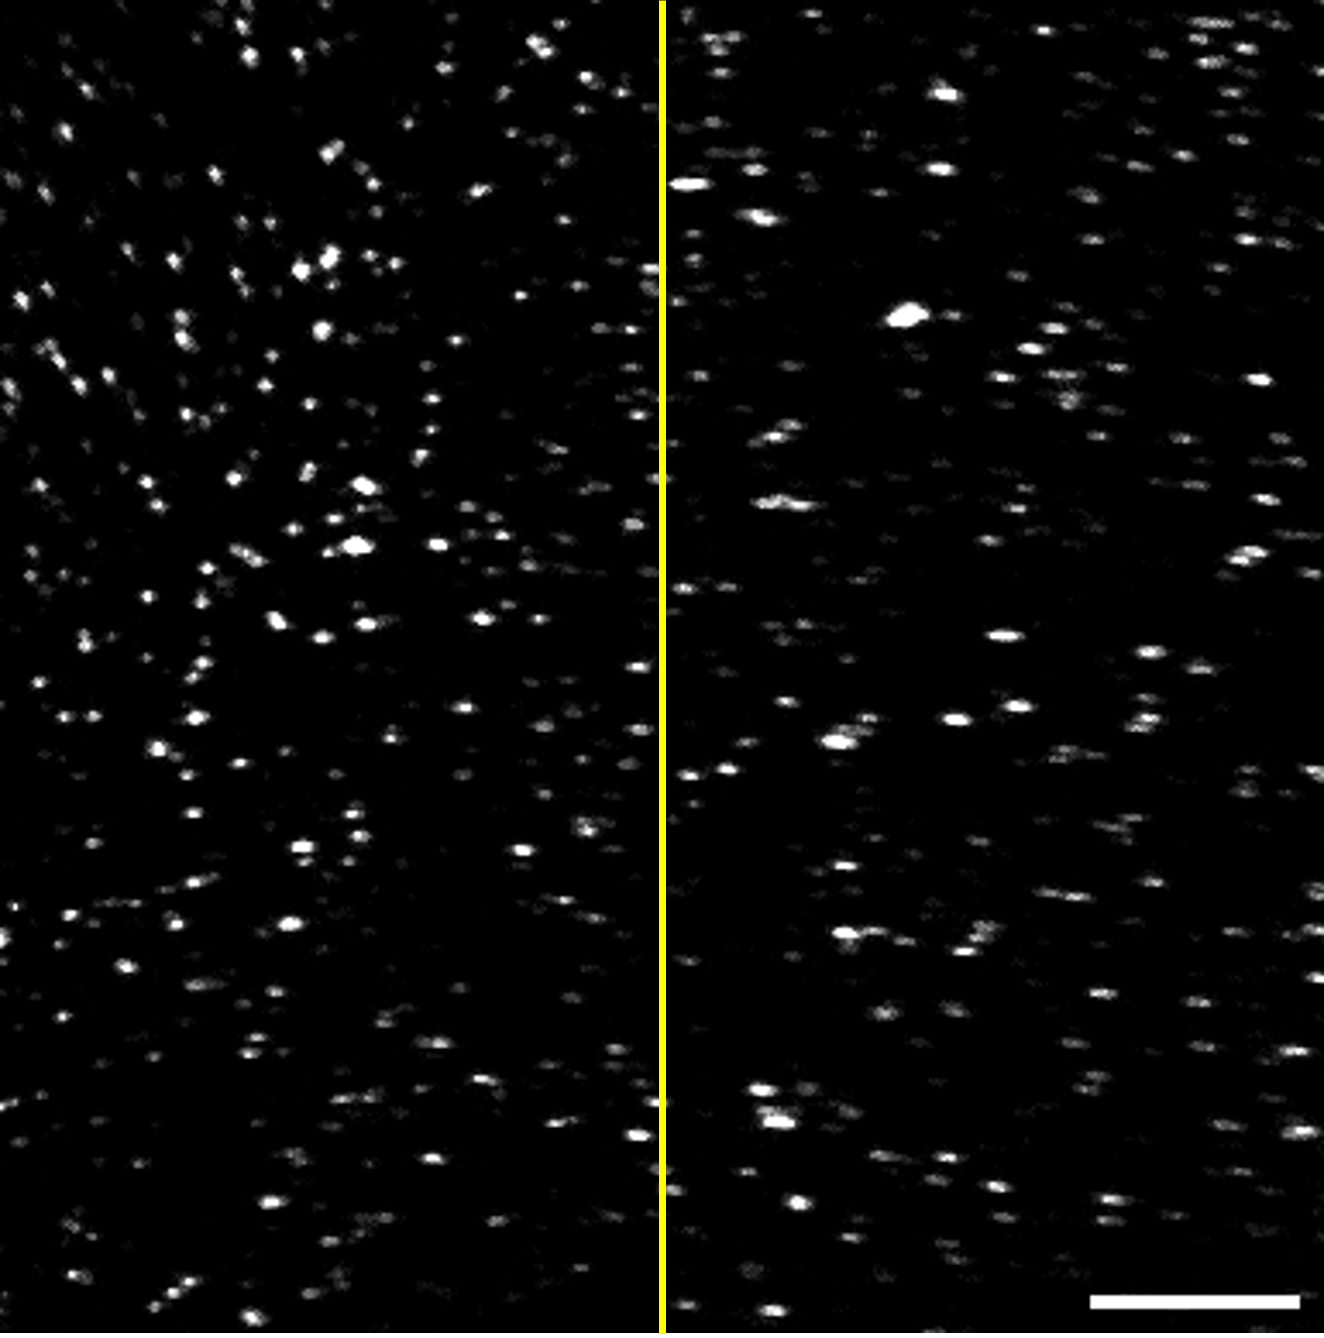
\includegraphics[width=0.6\linewidth]{Images/astigma2.png}
        \caption{\textbf{Uneven aberration and astigmatisms in adjacent regions imaged from mounted agarose bead sample.} Scale bar = 200 micron, yellow line marks clear boundary between adjacent normal and aberration regions. Image acquired using ImageJ software.}
    \end{subfigure}
    \medskip
    
    \begin{subfigure}[t]{0.75\textwidth}
        \centering
        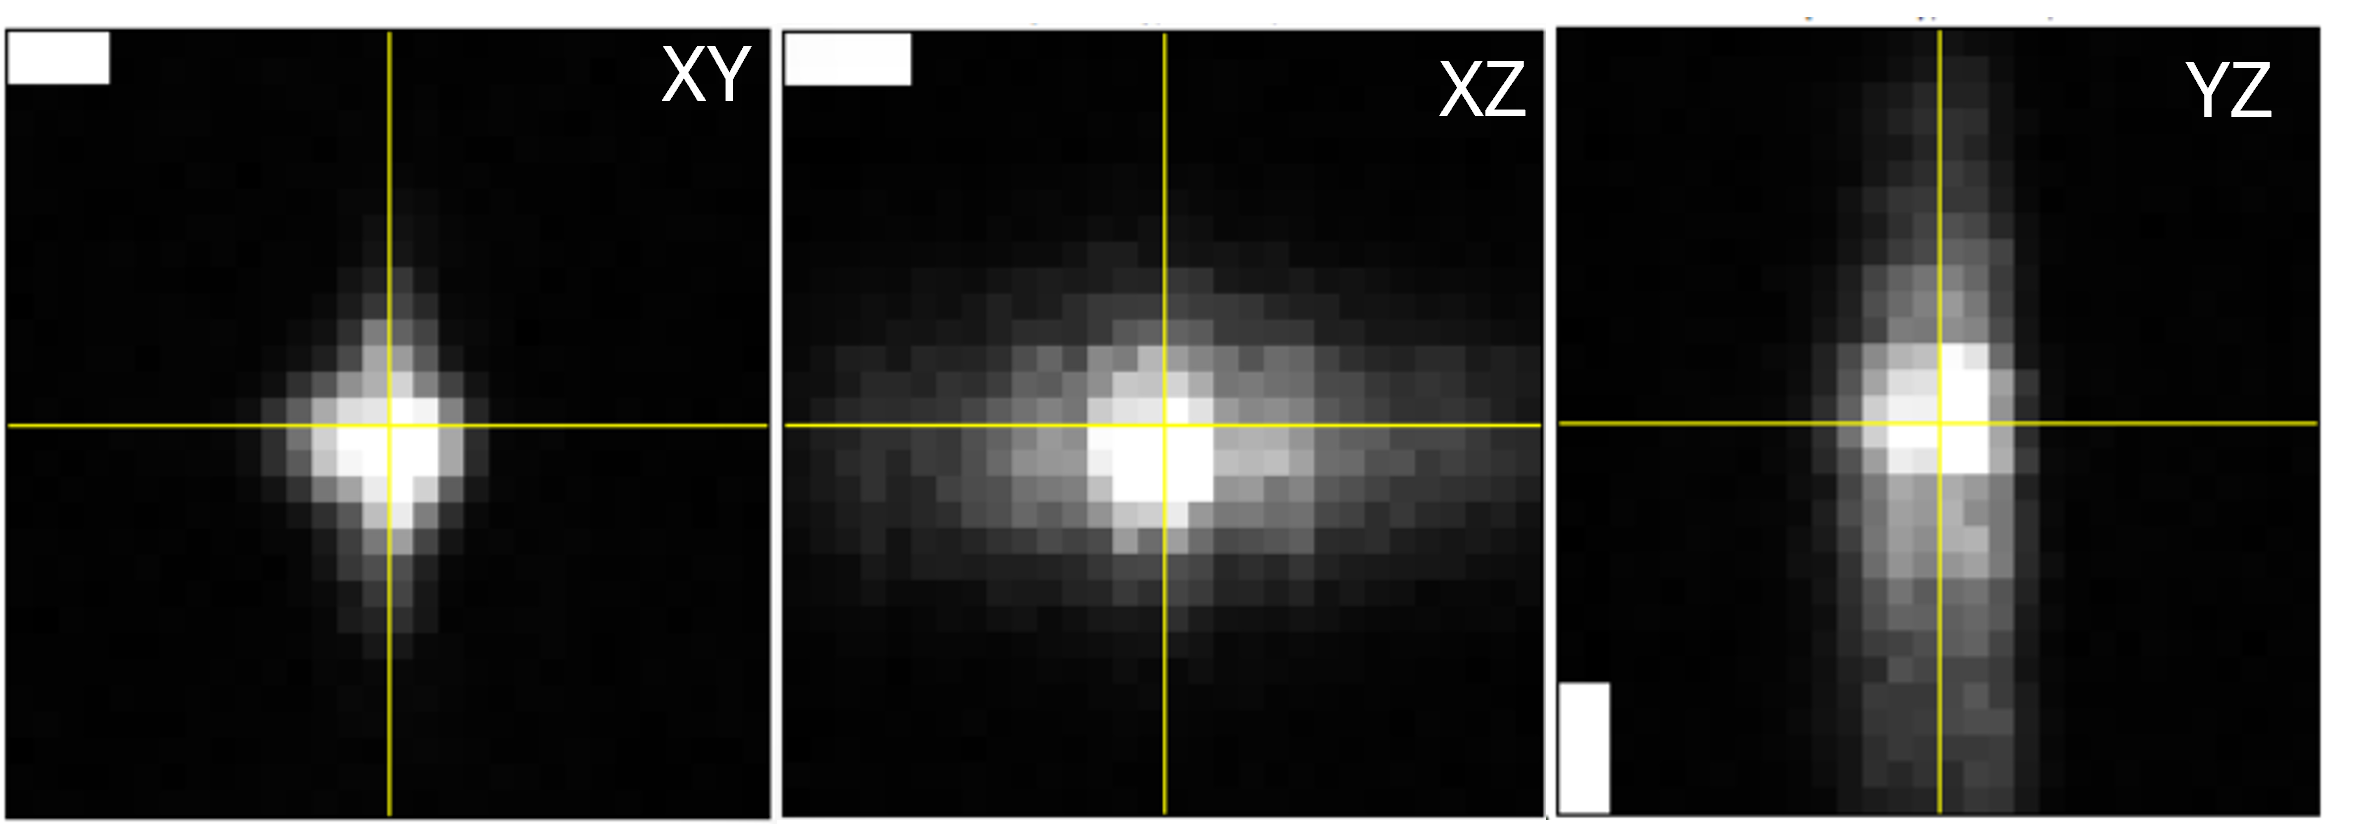
\includegraphics[width=0.8\linewidth]{Images/astigma1.png}
        \caption{\textbf{Astigmatism seen in an individual bead In XY, XZ, and YZ planes.} Scale Bars = 5 micron, Yellow Lines Mark Axis Midpoints. Image set acquired by Ahmed Elnageh using ImageJ software}
    \end{subfigure}
        
    \caption{\textbf{Image aberrations encountered during system characterization testing.} Overview image (A) and individual bead images (B).}
\end{figure}

Several measures and modifications were made to the design of the mounts (see Appendix 1) and the application of the silicone sealant was streamlined and made consistent across all samples mounted to mitigate the severity of these astigmatisms and aberrations in the images acquired. While these measures were unable to eliminate the issue entirely, the streamlining and optimization of the mount design and mounting protocol were able to reduce the variability of the issue and allow for more consistent characterization results to be acquired, allowing for more effective post-processing mitigation of optical aberrations to be performed. 

In addition to the external force applied by the quartz glass against the mount frame, it is anticipated that any warping or curling of the tissue held within the mount (see Chapter 3.3.2) will contribute additional force onto the surface of the slides as the flattened out tissue will press against the quartz glass as it tries to return to its curled state. While this additional force was not present in bead samples used for characterization testing, it remains a possibility that compounds the importance of avoiding any such curling in cleared tissue sample from occurring during implementation of this imaging pipeline.

\subsubsection{\textit{Considerations On Data Processing}}

One considerable advantage seen in the no shear processing method compared to the shear method is the considerable reduction in processing time and file sizes that results from the no shear method. Comparisons in file sizes and processing times are shown in Figure 4.12.

\begin{figure}[H]
    \centering
        \begin{subfigure}[t]{0.4\textwidth}
        \centering
        \begin{tikzpicture}
                \begin{axis}
                [
                scale = 0.85,
                xlabel = Raw Data File Size (GB),
                ylabel = Processed Data File Size (GB),
                xmin = 0,
                xmax = 18,
                ymax= 40,
                ymin = 0
                ]
                \addplot table {Data/Noshearfilesize.tex}
                ;
                \addplot table {Data/Shearfilesize.tex}
                        ; 
                \end{axis}
            \end{tikzpicture}
        \caption{\textbf{Change in file size of data after image processing}.}
        \label{fig:enter-label}
        \end{subfigure}
        \hspace{2em}
        ~
        \begin{subfigure}[t]{0.4\textwidth}
        \centering
         \begin{tikzpicture}
                \begin{axis}
                [
                scale = 0.85,
                xlabel = Input File Size (GB),
                ylabel = Processing Time (s),
                xmin = 0,
                xmax = 14,
                ymax= 300,
                ymin = 0
                ]
                \addplot table {Data/NoShearTime.tex}
                ;
                \addplot table {Data/ShearTime.tex}
                ; 
                \end{axis}
            \end{tikzpicture}
        \caption{\textbf{Change in affine transform processing time to input file size}.}
        \label{fig:enter-label}
        \end{subfigure}
    \caption{\textbf{Comparison of data processing files size and processing times}. Blue lines indicate trend for no shear data, red lines indicates trend for shear data.}
    \label{fig:enter-label}
\end{figure}

In comparison to the sheared processed data files, which increases in sizes by a factor of 4.24$\pm$0.07 (average$\pm$SD) , the no shear processed data files actually reduces the size of the original raw data file by a factor of 0.75$\pm$0.004. This leads to the file size of shear processed files being larger than the no-shear data files by a factor of 5.63$\pm$0.10. 

With regard to processing times, the sheared data on average was able to perform the affine transformation on the raw data at a rate of 22.53$\pm$0.33 milliseconds per GB. In comparison, the no shear process was able to perform the same image processing task at a faster rate with an average processing time of 13.32$/pm$0.18 milliseconds per GB. This equates to the no shear processing reducing the time required to process images by a factor of 1.69$\pm$0.03 compared to shear method.

These findings are of particular importance as the limited memory storage space in the PC operating the mesoSPIM proved to be a considerable challenge that can delay the recording and processing of data if not properly managed in a timely manner. To resolve this issue, any and all means by which the amount of memory and processing time required for a given tissue could be reduced without sacrificing image fidelity should be explored and implemented. Further discussion of specific measures considered throughout this project will be detailed in Chapter 6.

\section{Chapter Summary}

The final piece of the cardiac tissue imaging pipeline, customized sample mounting and data processing, was detailed in the first half of this chapter. The second half details the characterization experiments used to determine the achievable axial and lateral resolutions using inner cuvettes for both CLARITY and CUBIC-L/RA. In addition, the custom mounting and data processing methods (shear, no shear) used for CLARITY cleared slices were characterize to determine the loss in image fidelity incurred as a result of the oblique imaging methods deployed. The results obtained showed the no shear method of volume reconstruction of oblique mounted tissues as the superior method compared to sheared method. This is due to the no shear methods improving resolution in all spatial axes and allowing for the processing of image data with greater speed and smaller file sizes compared to sheared processing. As such, no shear data processing will be utilized in all subsequent analysis of cleared cardiac tissue. This, along with the rest of now fully described tissue imaging pipeline, will prove instrumental in the next chapter. Chapter 5 will present three cardiovascular research projects in which the completed and characterized cardiac tissue imaging pipeline was implemented from start to end, demonstrating the feasibility of utilizing the pipeline in current and future research into cardiac tissue structure.